\documentclass[11pt,a4paper]{article}
\usepackage{kotex}
\usepackage{amsmath,amssymb,amsfonts,amsthm}
\usepackage{graphicx}
\usepackage{booktabs}
\usepackage{algorithm}
\usepackage{algorithmic}
\usepackage{hyperref}
\usepackage{xcolor}
\usepackage{geometry}
\usepackage{tikz}
\usepackage{pgfplots}
\usepackage{float}
\usepackage{subcaption}
\usetikzlibrary{shapes.geometric, arrows, positioning, fit, calc, backgrounds}
\pgfplotsset{compat=1.17}
\geometry{margin=2.5cm}

\newtheorem{theorem}{정리}
\newtheorem{lemma}{보조정리}
\newtheorem{definition}{정의}

\DeclareMathOperator*{\argmax}{arg\,max}
\DeclareMathOperator*{\argmin}{arg\,min}
\DeclareMathOperator*{\E}{\mathbb{E}}
\DeclareMathOperator*{\CVaR}{\mathrm{CVaR}}
\DeclareMathOperator*{\VaR}{\mathrm{VaR}}

\title{\textbf{STAIR-RL: Semantic-Token Augmented Investment Reinforcement Learning\\for Cryptocurrency Portfolio Management}}
\author{
  Sihoon Kim \\
  \small Department of Electrical and Computer Engineering \\
  \small Seoul National University \\
  \small \texttt{bb9876543@snu.ac.kr}
}
\date{December 2025}

\begin{document}

\maketitle

\begin{abstract}
본 프로젝트는 STAIR-RL (\textbf{S}emantic-\textbf{T}oken \textbf{A}ugmented \textbf{I}nvestment \textbf{R}einforcement \textbf{L}earning) 프레임워크를 구현하고 분석한다.
STAIR-RL은 대규모 언어 모델(LLM)의 의미적 토큰을 전통적인 수치 특징과 결합하여 암호화폐 포트폴리오 관리를 위한 강화학습 에이전트를 학습한다.
핵심 기여는 다음과 같다: (1) information-theoretic 기반의 token selection mechanism인 TERC (Transfer Entropy Relevance Criterion), (2) dynamic semantic gating을 통한 noise filtering, (3) CQL-SAC에서 PPO-CVaR로의 two-stage offline-online transfer learning, (4) CVaR constraint를 통한 tail risk 관리.
본 보고서에서는 POMDP formulation, Late Fusion architecture, information-theoretic analysis, 그리고 implementation detail을 체계적으로 다룬다.
\end{abstract}

\vspace{0.5em}
\noindent\textbf{코드 저장소}: \url{https://github.com/menschhelt/STAIR-RL}

%==============================================================================
\section{서론}
%==============================================================================

\subsection{연구 배경}

2022년 Terra/Luna 붕괴와 FTX 파산 사태는 암호화폐 시장에서 테일 리스크(tail risk) 관리의 중요성을 극명하게 보여주었다.
불과 며칠 사이에 시가총액 수백억 달러가 증발했고, 이는 전통적인 위험 중립적(risk-neutral) 투자 전략의 한계를 드러냈다.

기존의 강화학습 기반 포트폴리오 관리 방법론은 이러한 극단적 상황에 대응하기 어렵다.
대부분의 RL 알고리즘이 기대 수익만을 최대화하기 때문에, 99.9\% 손실 같은 테일 이벤트는 학습 목표에 거의 영향을 미치지 않는다.
더욱이 기존 연구들은 가격과 거래량 같은 정형 데이터에만 의존하여, 규제 발표나 해킹 뉴스 같은 시장 급변의 전조를 포착하지 못한다.
암호화폐 시장의 비정상성(non-stationarity)---시장 레짐의 급격한 전환, 규제 환경의 변화, 새로운 자산군의 등장---은 오프라인에서 학습된 정책을 빠르게 무력화시킨다.

최근 대규모 언어 모델(LLM)의 발전은 이러한 한계를 극복할 새로운 가능성을 열었다.
FinBERT, CryptoBERT 같은 금융 특화 언어 모델은 뉴스와 소셜 미디어에서 시장 심리와 이벤트 정보를 추출할 수 있다.
그러나 LLM 출력을 강화학습에 \textit{효과적으로} 통합하는 방법론은 아직 체계화되지 않았으며, 단순히 임베딩을 연결하는 것만으로는 노이즈가 신호를 압도할 위험이 있다.

\subsection{핵심 연구 질문}

본 프로젝트는 다음 질문에 답한다:

\begin{quote}
\textit{``Semantic information이 sequential decision-making에 얼마나 valuable한가, 그리고 이를 어떻게 optimally 활용할 것인가?''}
\end{quote}

STAIR-RL은 이 질문에 대해 information-theoretic framework를 제시하며, semantic token의 value improvement가 conditional mutual information의 $O(\sqrt{I})$로 \textbf{upper bound}임을 이론적으로 보인다.

\subsection{주요 기여}

본 프로젝트는 네 가지 핵심 기여를 제시한다.

첫째, \textbf{TERC (Transfer Entropy Relevance Criterion)}는 transfer entropy를 기반으로 행동 결정에 실제로 유용한 semantic token만을 선택하는 information-theoretic criterion이다.
모든 토큰이 트레이딩에 도움이 되는 것은 아니며, 오히려 무관한 정보는 학습을 방해할 수 있다.
TERC는 submodular optimization을 통해 $(1-1/e) \approx 63.2\%$의 approximation guarantee를 제공한다.

둘째, \textbf{dynamic semantic gating} mechanism은 numerical market state에 따라 semantic information의 가중치를 자동으로 조절한다.
시장이 안정적일 때는 뉴스의 영향이 크지만, 급격한 가격 변동 시에는 수치적 시그널이 더 신뢰할 수 있다.
학습 가능한 게이트는 이러한 상황적 판단을 데이터로부터 학습한다.

셋째, \textbf{two-stage transfer learning} pipeline은 offline과 online 학습의 장점을 결합한다.
CQL-SAC로 18개월 오프라인 데이터에서 안전한 초기 정책을 학습한 후, PPO-CVaR로 18개월 온라인 학습 데이터에서 최근 시장에 적응시킨다.
이 접근은 충분한 탐색 없이 위험한 행동을 취하는 것을 방지하면서도 시장 변화에 대응할 수 있게 한다.

넷째, \textbf{CVaR constraint}는 Lagrangian dual method를 통해 tail risk를 명시적으로 제어한다.
기대 수익 최대화만으로는 ``블랙 스완'' 이벤트에 취약하지만, CVaR 제약은 최악의 5\% 시나리오에서도 손실을 제한한다.

%==============================================================================
\section{문제 분석 및 모티베이션}
%==============================================================================

본 절에서는 기존 RL 기반 암호화폐 트레이딩 연구의 한계를 체계적으로 분석하고, STAIR-RL의 설계 동기를 설명한다.

\subsection{위험 중립성 문제}

대부분의 RL 알고리즘은 기대 누적 보상을 최대화하는 목적함수 $\max_\pi \mathbb{E}_\pi [\sum_{t=0}^{\infty} \gamma^t r_t]$를 최적화한다.
이 formulation은 return distribution의 평균만 고려하며, variance나 tail risk를 명시적으로 다루지 않는다.

문제는 암호화폐 시장에서 극단적 손실이 빈번하게 발생한다는 점이다.
2022년 Terra/Luna 사태에서는 불과 며칠 만에 99.9\% 이상의 value가 증발했다.
이러한 ``블랙 스완'' 이벤트는 기대값 기반 목적함수에서는 거의 무시되지만, 실제 포트폴리오에는 치명적이다.
연간 50\%의 기대 수익을 달성하더라도, 단 한 번의 99\% 손실은 회복 불가능한 결과를 초래한다.

그러나 이러한 극단적 이벤트가 완전히 예측 불가능한 것은 아니다.
Terra/Luna 붕괴 이전에도 소셜 미디어에서는 UST 디페깅 리스크, 앵커 프로토콜의 지속 불가능한 수익률, 그리고 알고리즘 스테이블코인의 death spiral 가능성에 대한 우려가 꾸준히 제기되었다.
마찬가지로 FTX 파산 직전에도 CoinDesk의 알라메다 대차대조표 보도, 바이낸스 CEO의 FTT 매도 발표 등 명확한 경고 신호가 존재했다.
전통 금융에서도 2008년 금융위기 이전 서브프라임 모기지에 대한 우려는 전문가 사이에서 공유되고 있었다.

이러한 관찰은 \textbf{뉴스, 소셜 미디어, 거시경제 지표}를 통해 블랙 스완 이벤트의 사전 경고 신호를 포착할 수 있음을 시사한다.
가격 데이터만으로는 ``갑작스러운'' 폭락처럼 보이는 사건도, 텍스트 데이터에서는 점진적인 불안 증가로 나타날 수 있다.
STAIR-RL의 멀티모달 접근법은 이러한 사전적 신호를 활용하여 극단적 리스크를 회피하는 것을 목표로 한다.

\subsection{Non-stationarity와 Distribution Shift}

암호화폐 시장은 전통 금융 시장보다 훨씬 빠르게 변화한다.
시장 레짐(상승장/하락장/횡보장)이 수주 단위로 전환되고, 규제 환경은 예고 없이 급변한다.
2021년 중국의 채굴 금지, 2023년 SEC의 거래소 규제 강화 같은 이벤트는 시장 역학을 근본적으로 바꾸었다.
여기에 DeFi, NFT, Meme 코인 같은 새로운 자산군이 계속 등장하면서, 과거 데이터로 학습한 패턴이 빠르게 무효화된다.

이러한 분포 이동(distributional shift) 문제로 인해, 오프라인에서 아무리 좋은 성능을 보인 정책도 실제 배포 환경에서는 실패할 수 있다.
STAIR-RL의 2단계 전이 학습은 이 문제에 대응하기 위해 설계되었다.

\subsection{Spurious Correlations}

101개의 Alpha factor와 768차원 LLM embedding을 사용하면, high-dimensional feature space에서 RL agent가 spurious correlations를 학습할 위험이 있다.
특정 시간대에만 유효한 패턴, 소수 이벤트에 대한 과적합, 우연히 수익과 상관된 무관한 특징 등이 그 예이다.

Semantic information은 이러한 spurious correlations를 완화할 수 있다.
``SEC가 거래소를 조사한다''는 뉴스는 가격 하락의 \textit{원인}에 가까운 정보이며, 단순한 가격 패턴보다 더 일반화 가능하다.
그러나 모든 semantic token이 유용한 것은 아니므로, TERC를 통한 selection이 필수적이다.

\subsection{LLM 활용의 기술적 과제}

LLM을 실시간 트레이딩에 적용하려면 여러 기술적 과제를 해결해야 한다.
GPT-4 수준 모델의 추론 시간은 수 초에 달하며, 이는 5분봉 트레이딩에서도 상당한 지연이다.
또한 언어적 감성(``positive''/``negative'')과 금융적 함의가 항상 일치하지는 않는다---``금리 인상''이라는 뉴스는 언어적으로 중립적이지만 위험 자산에는 부정적이다.

STAIR-RL은 이 문제들을 두 가지 방식으로 해결한다.
첫째, 사전 계산된 FinBERT/CryptoBERT 임베딩을 사용하여 추론 지연을 제거한다.
둘째, TERC와 동적 게이팅을 통해 유용한 정보만을 선별하고 상황에 맞게 가중치를 조절한다.

%==============================================================================
\section{문제 정식화: POMDP}
%==============================================================================

\subsection{부분 관측 마르코프 결정 과정}

암호화폐 포트폴리오 관리 문제를 POMDP로 정식화한다:

\begin{definition}[POMDP]
POMDP $\mathcal{M} = (\mathcal{S}, \mathcal{A}, \mathcal{O}, \mathcal{T}, \mathcal{Z}, r, \gamma)$는 다음으로 구성된다:
\begin{itemize}
    \item $\mathcal{S}$: 상태 공간 (잠재 시장 레짐 포함)
    \item $\mathcal{A} = [-1, 1]^N$: 행동 공간 (N개 자산의 포트폴리오 가중치)
    \item $\mathcal{O}$: 관측 공간 (수치적 특징 + 의미적 토큰)
    \item $\mathcal{T}: \mathcal{S} \times \mathcal{A} \rightarrow \Delta(\mathcal{S})$: 전이 확률
    \item $\mathcal{Z}: \mathcal{S} \rightarrow \Delta(\mathcal{O})$: 관측 확률
    \item $r: \mathcal{S} \times \mathcal{A} \rightarrow \mathbb{R}$: 보상 함수 (상세 설계는 \ref{eq:reward}절 참조)
    \item $\gamma \in (0, 1)$: 할인율
\end{itemize}
\end{definition}

\subsection{부분 관측 문제}

에이전트는 진정한 상태 $s_t$를 직접 관측할 수 없다.
진정한 상태에는 다음이 포함된다:
\begin{itemize}
    \item 현재 시장 레짐 (상승장/하락장/횡보장)
    \item 다른 참여자들의 포지션과 의도
    \item 미공개 정보 (내부자 거래, 규제 계획 등)
\end{itemize}

에이전트가 관측하는 것은 $o_t = (F_t, H_t, x_t^{\text{port}})$로 구성된다:
\begin{itemize}
    \item $F_t \in \mathbb{R}^{N \times d_F}$: 수치적 팩터 (Alpha 101)
    \item $H_t \in \mathbb{R}^{d_H}$: 의미적 임베딩 (FinBERT, CryptoBERT)
    \item $x_t^{\text{port}} \in \mathbb{R}^{N+2}$: 현재 포트폴리오 상태
\end{itemize}

\subsection{Belief State의 Implicit Approximation}

POMDP의 optimal policy는 belief state $b_t = P(s_t \mid o_{1:t})$의 함수이다.
그러나 continuous state space에서 명시적 belief state 계산은 intractable하다.

본 연구에서는 deep POMDP 문헌의 표준적 접근을 따라, neural network가 관측 이력으로부터 \textbf{implicit하게 sufficient statistics를 학습}한다고 가정한다:
\begin{equation}
z_t = f_\theta(o_{1:t}) \approx \phi(b_t)
\end{equation}
여기서 GRU의 hidden state와 Attention mechanism이 belief state $b_t$의 sufficient statistics $\phi(b_t)$를 근사한다.

구체적으로, PriceTransformerEncoder가 OHLCV sequence를 인코딩하고, CrossAlphaAttention과 CrossAssetAttention이 feature 간 관계를 학습하며, 최종 GRU가 temporal aggregation을 수행한다.
이러한 구조는 명시적 belief update 없이도 과거 관측 이력을 효과적으로 요약한다.

\textbf{이론과 구현의 연결}: 섹션 \ref{sec:info_theory}의 information-theoretic analysis는 이상적인 POMDP belief state를 가정하지만, 실제 구현에서는 위의 implicit approximation을 사용한다.
이 gap의 정당성과 한계는 섹션 \ref{sec:theoretical_limits}에서 상세히 논의한다.

\subsection{CVaR 제약 목적함수}

기대 수익 최대화에 리스크 제약을 추가한다.
우선, 손실(Loss)을 $L = -R^{\text{port}}$로 정의한다 (양수 = 손실).

\begin{definition}[CVaR]
신뢰 수준 $\alpha \in (0, 1)$에 대해, Conditional Value at Risk는 다음과 같이 정의된다 (Rockafellar \& Uryasev, 2000):
\begin{equation}
\CVaR_\alpha(L) = \inf_{z \in \mathbb{R}} \left\{ z + \frac{1}{1-\alpha} \mathbb{E}[\max(L-z, 0)] \right\}
\end{equation}
이는 손실 분포의 상위 $(1-\alpha)$\% 꼬리 기대값(Expected Shortfall)을 의미한다.
$\alpha = 0.95$일 때, 최악의 5\% 시나리오에서의 평균 손실이다.
\end{definition}

제약 조건부 최적화 문제:
\begin{equation}
\max_\pi \mathbb{E}_\pi \left[ \sum_{t=0}^{\infty} \gamma^t r_t \right] \quad \text{s.t.} \quad \CVaR_\alpha(L) \leq \kappa
\end{equation}

Lagrangian dual problem으로 변환하면:
\begin{equation}
\min_{\lambda \geq 0} \max_\pi \mathcal{L}(\pi, \lambda) = \mathbb{E}_\pi[R] - \lambda \cdot (\CVaR_\alpha(L) - \kappa)
\end{equation}

%==============================================================================
\section{State 구성 상세}
%==============================================================================

\subsection{Numerical Features: Alpha 101}

Kakushadze (2016)의 ``101 Formulaic Alphas'' 논문에 기반한 수식 기반 팩터를 사용한다.
이 알파들은 OHLCV 데이터에 수학적 연산자를 조합 적용하여 생성되며, RSI나 MACD 같은 전통적 기술적 지표와는 근본적으로 다르다.

\textbf{Alpha 모델 선택의 근거}:
Alpha 팩터는 퀀트 투자 업계에서 초과수익률(알파)을 창출하기 위한 핵심 도구로 널리 활용되고 있다.
대표적으로 WorldQuant의 알파 리서치 플랫폼인 WorldQuant Brain에서는 수백만 개의 alpha 수식을 탐색하고 조합하여 투자 전략을 구성하며, 이는 alpha 기반 접근법의 실무적 유효성을 입증한다.
많은 퀀트 펀드와 연구자들이 여전히 alpha 모델을 시장 비효율성을 포착하고 벤치마크 대비 초과수익을 달성하기 위한 유효한 피처로 간주하고 있다.

특히 암호화폐 시장의 경우, 전통 금융 시장에 비해 기관급 투자자나 전문 시장 참여자의 비중이 상대적으로 낮아 시장 효율성이 떨어지는 것으로 알려져 있다.
이러한 시장 특성으로 인해 개별 alpha 신호의 예측력이 더욱 유의미하게 유지될 수 있으며, 본 연구에서 Alpha 101 팩터를 핵심 수치 피처로 채택한 주요 근거가 된다.

\begin{table}[h]
\centering
\caption{Alpha 101 Operations and Inputs}
\begin{tabular}{ll}
\toprule
\textbf{Category} & \textbf{Elements} \\
\midrule
Time-Series Ops & \texttt{ts\_rank}, \texttt{ts\_min}, \texttt{ts\_max}, \texttt{ts\_argmax}, \texttt{delay}, \texttt{delta} \\
Cross-Sectional Ops & \texttt{rank}, \texttt{scale}, \texttt{indneutralize} \\
Statistical Ops & \texttt{correlation}, \texttt{covariance}, \texttt{stddev}, \texttt{sum}, \texttt{product} \\
Transform Ops & \texttt{decay\_linear}, \texttt{signedpower}, \texttt{log}, \texttt{abs} \\
Input Data & \texttt{open}, \texttt{close}, \texttt{high}, \texttt{low}, \texttt{volume}, \texttt{vwap}, \texttt{returns} \\
\bottomrule
\end{tabular}
\end{table}

예시 알파 수식:
\begin{align}
\text{Alpha\#1} &= \text{rank}(\text{ts\_argmax}(\text{signedpower}(r < 0 \;?\; \sigma_{20}(r) : c, 2), 5)) - 0.5 \\
\text{Alpha\#6} &= -\text{correlation}(\text{open}, \text{volume}, 10)
\end{align}

각 알파는 자산별로 계산되어 $(N, 101)$ 형태의 텐서를 구성하고, 시간적 문맥을 위해 과거 $T$ 타임스텝을 유지하여 최종 형태는 $(T, N, 101)$이다.

\textbf{데이터 수집}:
Binance Futures의 5분봉 OHLCV 데이터는 오픈소스 트레이딩 봇 프레임워크인 \texttt{freqtrade}를 활용하여 수집하였다.
Binance Futures에서 제공하는 모든 perpetual contract의 5분봉 데이터를 feather 형식으로 다운로드한 후, 본 연구의 데이터 파이프라인에 적합한 양식으로 변환하였다.

\textbf{Alpha 전처리 (Cross-Sectional Normalization)}:
Raw alpha 값은 자산 간 스케일 차이가 크고 시간에 따라 분포가 변동하므로, 매 시점마다 다음 두 단계의 cross-sectional normalization을 적용한다:
\begin{enumerate}
    \item \textbf{Cross-sectional mean neutralization}: 각 시점 $t$에서 자산 간 평균을 0으로 조정한다.
    \begin{equation}
    \tilde{\alpha}_{t,i}^{(k)} = \alpha_{t,i}^{(k)} - \frac{1}{N}\sum_{j=1}^{N} \alpha_{t,j}^{(k)}
    \end{equation}
    이는 long-short portfolio 전략의 기본 가정으로, 시장 전체의 방향성이 아닌 자산 간 상대적 강도를 포착한다.

    \item \textbf{$L_1$ normalization}: 각 시점에서 alpha 벡터의 절댓값 합을 1로 정규화한다.
    \begin{equation}
    \hat{\alpha}_{t,i}^{(k)} = \frac{\tilde{\alpha}_{t,i}^{(k)}}{\sum_{j=1}^{N} |\tilde{\alpha}_{t,j}^{(k)}| + \epsilon}
    \end{equation}
    여기서 $\epsilon = 10^{-8}$은 수치 안정성을 위한 상수이다.
\end{enumerate}

이러한 전처리를 통해 모든 알파가 동일한 스케일로 정규화되며, 에이전트가 자산 간 상대적 매력도를 학습하는 데 집중할 수 있다.
모든 알파의 cross-sectional 연산에는 매 시점에 존재하는 심볼만 사용하도록 하였으며, 모델에는 \ref{sec:universe}절에서 설명하는 유니버스 선정 방식에 따라 선택된 Top-20 심볼들의 알파 신호가 입력된다.

\subsection{Semantic Features}

본 연구에서는 두 종류의 LLM 임베딩을 활용하여 semantic information을 포착한다.

\subsubsection{FinBERT (뉴스)}
FinBERT 임베딩은 GDELT API와 주요 암호화폐 뉴스 사이트 웹 스크래핑을 통해 수집한 금융 뉴스로부터 추출된다.
5분 단위로 집계된 뉴스 헤드라인이 입력되어 768차원 임베딩 벡터를 생성하며,
Top-20 자산 관련 뉴스의 가중 평균으로 전처리된다.

\subsubsection{CryptoBERT (소셜)}
CryptoBERT 임베딩은 Nostr 탈중앙화 소셜 네트워크의 실시간 포스트로부터 추출되어 768차원 벡터를 생성한다.
소셜 데이터의 특성상 데이터가 없는 시점이 존재하므로, 신호 가용성 마스크 $m_t \in \{0, 1\}$를 통해 부재 시 영벡터로 처리한다.

두 임베딩 모두 TextProjection MLP를 통해 64차원으로 압축된다:
\begin{equation}
h_{\text{text}} = \text{MLP}_{768 \rightarrow 256 \rightarrow 64}(h_{\text{BERT}})
\end{equation}

\subsection{Global Market Features}

28개의 거시경제 지표를 포함하며, yfinance API와 FRED (Federal Reserve Economic Data) API를 통해 수집한다:

\begin{table}[h]
\centering
\caption{Global Market Features}
\begin{tabular}{lccp{6cm}}
\toprule
\textbf{Category} & \textbf{Count} & \textbf{Source} & \textbf{Indicators} \\
\midrule
Interest Rates & 5 & FRED & Fed Funds Rate, 2/10/30Y Treasury Yields, LIBOR \\
Volatility & 3 & yfinance & VIX, MOVE Index, High-Yield Spread \\
Equity Markets & 5 & yfinance & S\&P 500, NASDAQ, Emerging Markets Index \\
Commodities & 5 & yfinance & Gold, Crude Oil, Copper, Dollar Index \\
Fama-French (Crypto-adapted) & 5 & Crypto Universe & MKT\_RF, SMB, HML, RMW, CMA \\
Macroeconomic & 5 & FRED & M2 Money Supply, Unemployment, CPI, Housing Price \\
\bottomrule
\end{tabular}
\end{table}

\subsection{Portfolio State}

현재 포트폴리오 상태 $x_t^{\text{port}} \in \mathbb{R}^{N+2}$:
\begin{itemize}
    \item 현재 가중치: $w_t \in [-1, 1]^N$ (숏 포지션 허용)
    \item 레버리지 비율: $\ell_t = \sum_i |w_{t,i}|$
    \item 현금 비율: $c_t = 1 - \sum_i |w_{t,i}|$ (레버리지 없을 시)
\end{itemize}

\subsection{State 설계 근거 및 기대 효과}

각 State 구성 요소의 설계 의도와 에이전트가 학습하기를 기대하는 판단 능력을 설명한다.
State는 크게 \textbf{시계열 처리 경로}(GRU 통과)와 \textbf{스냅샷 경로}(MLP만 통과)로 나뉜다.

\begin{table}[h]
\centering
\caption{State 구성 요소별 설계 의도 요약}
\begin{tabular}{lccp{5.5cm}}
\toprule
\textbf{Feature} & \textbf{차원} & \textbf{GRU} & \textbf{기대 판단} \\
\midrule
Market State & 36/asset & $\times$ & 캔들 패턴, 다중 시간 모멘텀 \\
Alpha 101 & 101/asset & $\checkmark$ & 기술적 신호, 이상 탐지 \\
OHLCV Seq & 360/asset & $\checkmark$ & 6시간 추세, 변동성 레짐 \\
News (FinBERT) & 768$\to$64 & $\checkmark$ & 규제/이벤트 전조 \\
Social (CryptoBERT) & 768$\to$64 & $\checkmark$ & FOMO/FUD, 루머 \\
Macro Factors & 23 & $\times$ & Risk-on/off, 유동성 \\
Fama-French (Crypto) & 5 & $\times$ & 크립토 스타일 로테이션 \\
Portfolio State & 22 & $\times$ & Lazy trading, 레버리지 관리 \\
\bottomrule
\end{tabular}
\end{table}

\subsubsection{Market State (36차원/자산) - 가격 기반 특징}

Market State는 36개 특징으로 구성되며, 캔들스틱 정보와 다중 시간 스케일의 수익률을 포함한다.
첫 번째 특징 $f_0 = \log(c_t / o_t)$는 캔들 바디 방향(양봉/음봉)을 나타내고,
$f_1 = \log(h_t / c_t)$과 $f_2 = \log(c_t / l_t)$는 각각 위꼬리와 아래꼬리 길이로서 매도/매수 압력을 반영한다.
$f_3 = \log(1 + v_t) / 20$은 정규화된 거래량, $f_4 = p_t / 10000$은 정규화된 가격이다.
나머지 $f_{5:36}$은 lag 1부터 31까지의 과거 수익률 $r_{t-\text{lag}} \times \sqrt{\text{lag}}$로 구성된다.

Log return 변환은 시계열 정상성(stationarity)을 확보하여 학습 안정성을 높이며,
$\sqrt{\text{lag}}$ 스케일링은 분산이 시간 스케일에 비례하는 특성($\sigma^2 \propto t$)을 정규화한다.

이러한 lag 구조를 통해 에이전트는 다양한 시간 스케일의 모멘텀을 학습할 수 있다.
단기 lag(1--5)는 즉각적인 추세 연속성을, 중기 lag(6--20)는 추세의 강도를,
장기 lag(21--31)는 평균 회귀 가능성을 포착한다.
또한 캔들스틱의 바디와 꼬리 비율로부터 도지(doji), 망치형 등 기술적 전환점 패턴을 인식할 수 있다.

\subsubsection{Alpha 101 (101차원/자산)}

Kakushadze (2016)의 ``101 Formulaic Alphas''는 헤지펀드에서 검증된 퀀트 팩터 모음이다.
단순 기술적 지표(RSI, MACD)와 달리 \texttt{ts\_rank}, \texttt{correlation}, \texttt{decay\_linear} 등 복잡한 연산자를 조합하여 비선형 패턴을 포착한다.

에이전트는 이 팩터들로부터 다양한 트레이딩 신호를 학습할 수 있다.
예를 들어 Alpha\#53은 52주 신고점 근접도를 측정하여 모멘텀 또는 반전 타이밍을 포착하고,
Alpha\#41은 거래량 급변을 통해 유동성 이상을 탐지하며,
Alpha\#13은 가격-거래량 상관관계의 이탈로부터 반전 신호를 감지한다.

이 팩터들은 GRU를 통과하여 시계열 변화 패턴까지 학습하게 된다.
이를 통해 ``알파가 상승 추세일 때 매수''와 같은 동적 전략이 가능해진다.

\subsubsection{OHLCV Sequences (72$\times$5차원/자산)}

72개의 5분봉, 즉 6시간 분량의 가격 히스토리를 Transformer 인코더로 처리하여 장거리 의존성을 포착한 후 GRU로 시간 압축한다.

에이전트는 이 시퀀스로부터 추세 방향(상승/하락/횡보 레짐)을 식별하고,
변동성 레짐을 인식하여 고변동성 구간에서 포지션을 축소하는 전략을 학습할 수 있다.
또한 삼각 수렴, 이중 바닥 등의 차트 패턴을 암묵적으로 인식하여 기술적 분석 기반의 의사결정이 가능해진다.

\subsubsection{News Embeddings - FinBERT (768$\to$64차원)}

GDELT 뉴스의 FinBERT 임베딩은 시장 외부 정보를 포착한다.
가격 데이터만으로는 알 수 없는 규제, 해킹, 상장 등의 이벤트를 선반영할 수 있다는 점에서 중요하다.

에이전트는 이 임베딩으로부터 ``SEC 조사'', ``해킹 의혹'' 같은 급변 전조 키워드를 감지하고,
긍정/부정 뉴스 톤에 따라 포지션을 조정하는 전략을 학습할 수 있다.
특히 GRU를 통해 뉴스 톤의 변화 추세까지 학습하므로,
``부정적 뉴스가 연속 3일 증가''와 같은 시계열 패턴을 인식하여 선제적 대응이 가능해진다.

\subsubsection{Social Embeddings - CryptoBERT (768$\to$64차원)}

Nostr 탈중앙화 소셜 네트워크의 CryptoBERT 임베딩은 개인 투자자 심리를 반영한다.
공식 뉴스보다 루머와 커뮤니티 반응이 먼저 나타나는 경우가 많아, 선행 지표로서의 가치가 있다.

에이전트는 이 임베딩으로부터 ``달에 간다!'' 같은 FOMO(Fear of Missing Out)와 ``폭락 온다'' 같은 FUD(Fear, Uncertainty, Doubt)를 감지할 수 있다.
또한 뉴스에 반영되기 전의 소셜 버즈를 포착하여 초기 신호로 활용할 수 있다.
데이터 부재 시에는 Signal Mask $m_t \in \{0, 1\}$를 통해 영벡터로 처리한다.

\subsubsection{Macro Factors (23차원) + Fama-French (5차원)}

거시경제 지표는 시장 전체의 리스크 선호도를 결정하는 핵심 요인이다.
암호화폐는 대표적인 위험자산으로, 금리 인상기에는 자금이 이탈하고 유동성 확대기에는 유입되는 특성을 보인다.

에이전트는 금리 환경(DFF, DGS10)으로부터 Risk-on/off 상황을 판단하고,
VIX 지수로 시장 공포 수준을 평가하여 포지션 사이즈를 조절할 수 있다.
M2 통화량과 WALCL(연준 대차대조표)은 유동성 상황을 반영하여 암호화폐 수요를 예측하는 데 활용된다.

Fama-French 팩터는 전통적인 주식 시장이 아닌 암호화폐 유니버스에서 직접 계산된다.
SMB는 시가총액 기준, HML은 가격 모멘텀 기반 (B/M 대용), RMW는 거래량 기반 (수익성 대용), CMA는 변동성 기반 (투자 스타일 대용)으로 적응하였다.
이를 통해 암호화폐 시장 내의 대형/소형, 모멘텀/가치, 고변동성/저변동성 스타일 간 수익률 차이를 포착한다.

이 지표들은 월간 또는 주간 단위로 업데이트되므로 5분 단위 시계열 처리가 불필요하여 GRU를 통과하지 않는다.
현재 스냅샷만으로 ``금리 인상기'' 대 ``완화기''를 판단할 수 있다.
다만 매크로 추세 변화, 예를 들어 금리 피벗 시점의 학습은 이 구조로는 제한적이라는 한계가 있다.

\subsubsection{Portfolio State (22차원)}

현재 포지션 정보를 에이전트에게 제공하여 Lazy Trading을 유도한다.
자신이 이미 BTC 30\%를 보유 중임을 인식하지 못하면 불필요한 매수/매도가 반복되기 때문이다.

에이전트는 현재 가중치를 인식함으로써 포지션 변경 비용 대비 기대 이익을 평가하고,
과도한 레버리지를 회피하는 전략을 학습할 수 있다.
또한 일정 수준의 현금을 유지하여 급락 시 매수 기회를 포착할 여력을 확보하는 것도 가능해진다.

포지션 정보는 현재 스냅샷만 필요하므로 GRU를 통과하지 않는다.
과거 포지션 히스토리는 미래 의사결정에 직접적인 영향을 미치지 않기 때문이다.

%==============================================================================
\section{아키텍처}
%==============================================================================

\subsection{전체 구조: Late Fusion}

STAIR-RL은 Late Fusion 구조를 채택하여 각 모달리티를 독립적으로 인코딩한 후 후반부에서 결합한다.

\begin{figure}[h]
\centering
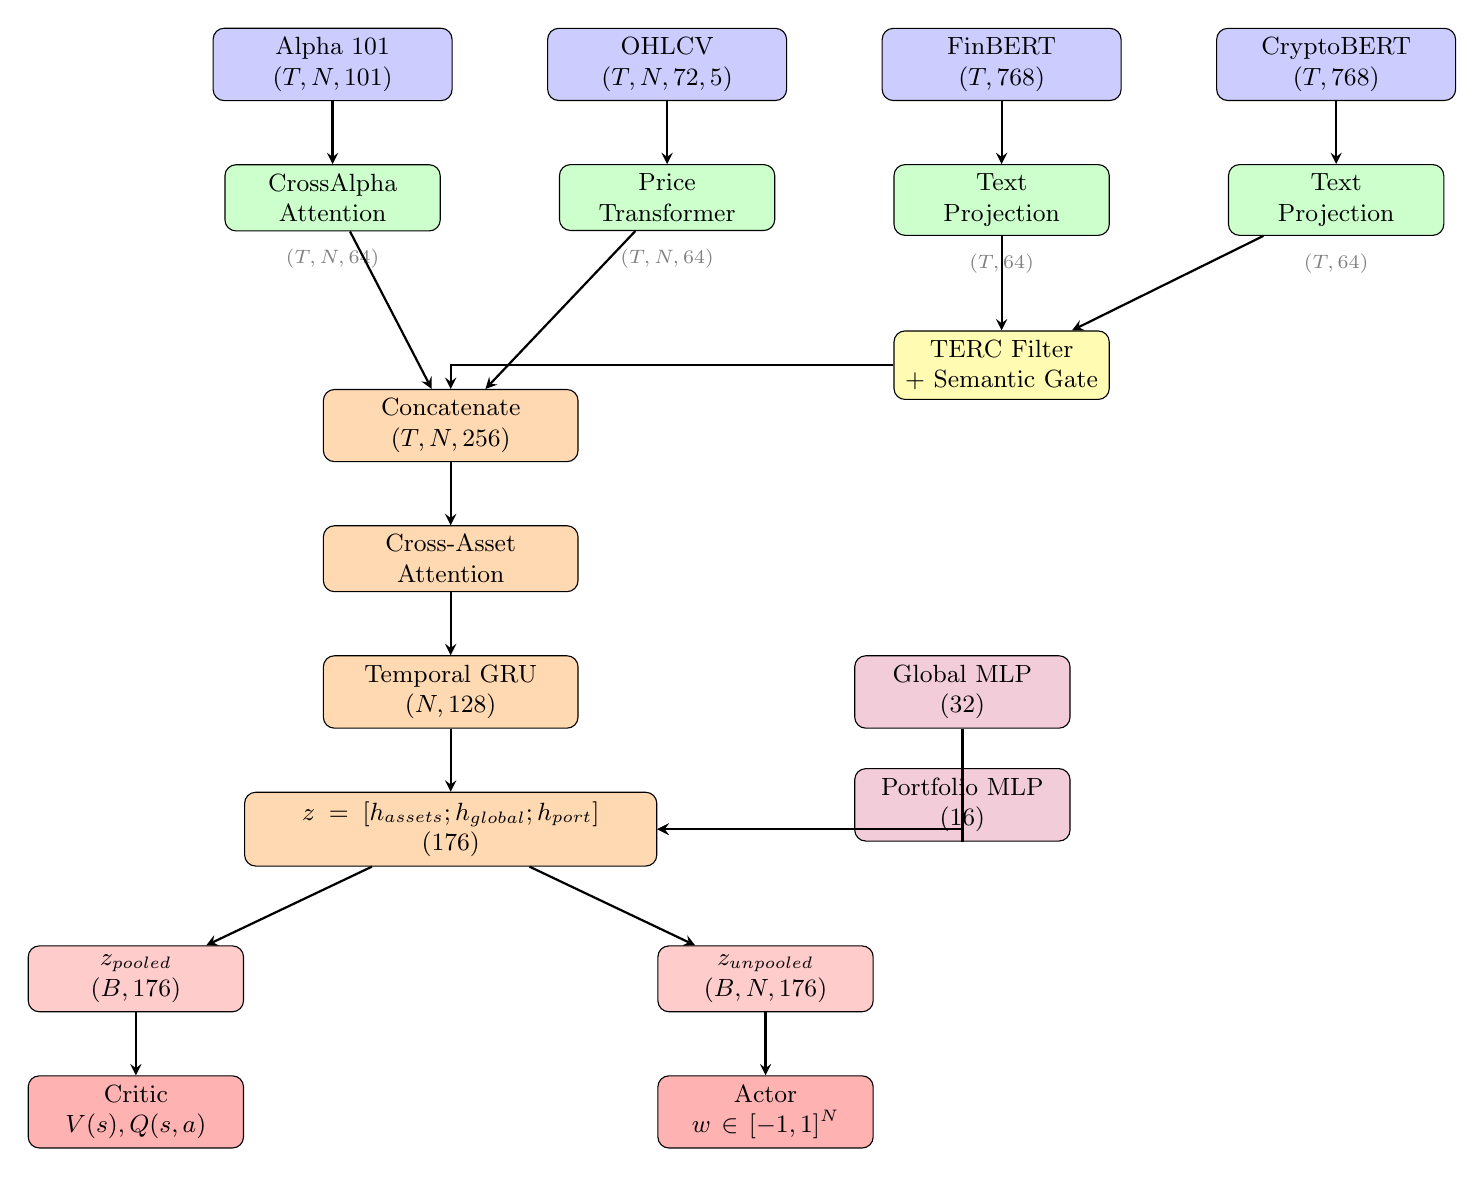
\begin{tikzpicture}[
    node distance=0.8cm and 1.2cm,
    block/.style={rectangle, draw, fill=blue!20, text width=2.8cm, text centered, rounded corners, minimum height=0.8cm, font=\small},
    encoder/.style={rectangle, draw, fill=green!20, text width=2.5cm, text centered, rounded corners, minimum height=0.7cm, font=\small},
    fusion/.style={rectangle, draw, fill=orange!30, text width=3cm, text centered, rounded corners, minimum height=0.8cm, font=\small},
    output/.style={rectangle, draw, fill=red!20, text width=2.5cm, text centered, rounded corners, minimum height=0.7cm, font=\small},
    arrow/.style={->, >=stealth, thick},
    label/.style={font=\scriptsize, text=gray}
]

% Input layer
\node[block] (alpha) {Alpha 101\\$(T,N,101)$};
\node[block, right=of alpha] (ohlcv) {OHLCV\\$(T,N,72,5)$};
\node[block, right=of ohlcv] (news) {FinBERT\\$(T,768)$};
\node[block, right=of news] (social) {CryptoBERT\\$(T,768)$};

% Encoder layer
\node[encoder, below=of alpha] (alpha_enc) {CrossAlpha\\Attention};
\node[encoder, below=of ohlcv] (price_enc) {Price\\Transformer};
\node[encoder, below=of news] (news_enc) {Text\\Projection};
\node[encoder, below=of social] (social_enc) {Text\\Projection};

% Dimension labels
\node[label, below=0.1cm of alpha_enc] {$(T,N,64)$};
\node[label, below=0.1cm of price_enc] {$(T,N,64)$};
\node[label, below=0.1cm of news_enc] {$(T,64)$};
\node[label, below=0.1cm of social_enc] {$(T,64)$};

% TERC and Gate
\node[encoder, below=1.2cm of news_enc, fill=yellow!30] (terc) {TERC Filter\\+ Semantic Gate};

% Fusion layer
\node[fusion, below=2cm of alpha_enc, xshift=1.5cm] (concat) {Concatenate\\$(T,N,256)$};

% Cross-asset attention
\node[fusion, below=of concat] (cross) {Cross-Asset\\Attention};

% Temporal GRU
\node[fusion, below=of cross] (gru) {Temporal GRU\\$(N,128)$};

% Global/Portfolio
\node[encoder, right=3.5cm of gru, fill=purple!20] (global) {Global MLP\\$(32)$};
\node[encoder, below=0.5cm of global, fill=purple!20] (port) {Portfolio MLP\\$(16)$};

% Final representation
\node[fusion, below=of gru, text width=5cm] (final) {$z = [h_{assets}; h_{global}; h_{port}]$\\$(176)$};

% Output heads
\node[output, below left=1cm and 0cm of final] (pooled) {$z_{pooled}$\\$(B, 176)$};
\node[output, below right=1cm and 0cm of final] (unpooled) {$z_{unpooled}$\\$(B, N, 176)$};

% Actor/Critic
\node[output, below=of pooled, fill=red!30] (critic) {Critic\\$V(s), Q(s,a)$};
\node[output, below=of unpooled, fill=red!30] (actor) {Actor\\$w \in [-1,1]^N$};

% Arrows - Input to Encoder
\draw[arrow] (alpha) -- (alpha_enc);
\draw[arrow] (ohlcv) -- (price_enc);
\draw[arrow] (news) -- (news_enc);
\draw[arrow] (social) -- (social_enc);

% Arrows - Encoder to TERC/Fusion
\draw[arrow] (alpha_enc) -- (concat);
\draw[arrow] (price_enc) -- (concat);
\draw[arrow] (news_enc) -- (terc);
\draw[arrow] (social_enc) -- (terc);
\draw[arrow] (terc) -| (concat);

% Arrows - Fusion flow
\draw[arrow] (concat) -- (cross);
\draw[arrow] (cross) -- (gru);
\draw[arrow] (gru) -- (final);
\draw[arrow] (global) |- (final);
\draw[arrow] (port) |- (final);

% Arrows - Output
\draw[arrow] (final) -- (pooled);
\draw[arrow] (final) -- (unpooled);
\draw[arrow] (pooled) -- (critic);
\draw[arrow] (unpooled) -- (actor);

\end{tikzpicture}
\caption{STAIR-RL Late Fusion 아키텍처. 각 모달리티는 독립적으로 인코딩된 후 Cross-Asset Attention과 GRU를 통해 결합된다. $z_{pooled}$는 Critic에, $z_{unpooled}$는 Actor에 입력된다.}
\label{fig:architecture}
\end{figure}

\subsection{모달리티별 인코더}

\subsubsection{CrossAlphaAttention}
101개 Alpha 팩터를 64차원으로 압축한다:
\begin{equation}
h_\alpha = \text{MultiHeadAttn}(\text{Linear}_{101 \rightarrow 64}(\text{alphas}))
\end{equation}

8-head self-attention으로 팩터 간 상호작용을 학습한다.

\subsubsection{PriceTransformerEncoder}
5분봉 OHLCV 시퀀스(72개 = 6시간)를 64차원으로 인코딩:
\begin{equation}
h_{\text{price}} = \text{MeanPool}(\text{TransformerEncoder}(\text{Linear}_{5 \rightarrow 64}(\text{OHLCV})))
\end{equation}

2-layer Transformer (4-head, FFN=128)를 사용한다.

\textbf{OHLCV 전처리 - Log Returns 차분}:
시계열 정상성(stationarity) 확보를 위해 raw 가격 대신 log returns를 사용한다:
\begin{align}
r_t^{\text{price}} &= \log(p_t / p_{t-1}) \times 100 \quad \text{(OHLC 각각)} \\
r_t^{\text{volume}} &= \log(v_t / v_{t-1}) \quad \text{(거래량 변화율)}
\end{align}

이 전처리가 필수인 이유는 세 가지이다.
첫째, raw 가격은 추세(trend)를 포함하여 non-stationary하지만 log returns는 평균 0 근처에서 stationary하다.
둘째, 100원 코인과 50,000달러 BTC를 동일한 스케일로 비교할 수 있는 스케일 불변성을 제공한다.
셋째, 여러 기간의 수익률을 단순 합산할 수 있는 가법성($\sum_t r_t = \log(p_T/p_0)$)이 있다.

스케일링 계수 100은 일반적인 5분봉 log returns ($\approx 0.001$)를 신경망에 적합한 범위 ($\approx 0.1$)로 조정한다.

\subsubsection{TextProjection}
768차원 BERT 임베딩을 64차원으로 압축:
\begin{equation}
h_{\text{text}} = \text{Linear}_{256 \rightarrow 64}(\text{ReLU}(\text{Linear}_{768 \rightarrow 256}(h_{\text{BERT}})))
\end{equation}

\subsection{Cross-Asset Attention}

$N$개 자산 간의 동적 상관관계를 학습한다:
\begin{equation}
h_{\text{cross}} = \text{MultiHeadAttn}(h_{\text{concat}}, h_{\text{concat}}, h_{\text{concat}})
\end{equation}

이를 통해 ``BTC가 움직일 때 ETH는 어떻게 반응하는가?'' 같은 자산 간 관계를 포착한다.

\subsection{이중 출력: $z_{pooled}$ vs $z_{unpooled}$}

핵심 설계 결정으로 두 가지 표현을 생성하여 Critic과 Actor에 각각 적합한 입력을 제공한다.

$z_{\text{pooled}} \in \mathbb{R}^{176}$는 자산 차원을 평균 풀링한 전역 표현이다:
\begin{equation}
z_{\text{pooled}} = [\text{MeanPool}_N(h_{\text{assets}}); h_{\text{global}}; h_{\text{port}}]
\end{equation}
이 표현은 포트폴리오 전체의 가치를 평가하는 Critic(value function)의 입력으로 사용된다.

반면 $z_{\text{unpooled}} \in \mathbb{R}^{N \times 176}$는 자산별 표현을 유지한다:
\begin{equation}
z_{\text{unpooled}} = [h_{\text{assets}}; \text{Broadcast}(h_{\text{global}}); \text{Broadcast}(h_{\text{port}})]
\end{equation}
이 표현은 개별 자산의 가중치를 결정해야 하는 Actor(정책 함수)의 입력으로 사용된다.

%==============================================================================
\section{Hierarchical Policy}
%==============================================================================

\subsection{Lazy Agent 설계}

STAIR-RL의 Actor는 ``Lazy Agent'' 방식을 채택한다.
명시적인 거래/보유 결정(Meta-Controller) 없이 Portfolio Head만으로 구성된다:

\begin{equation}
w_t = \tanh(\text{MLP}(z_{\text{unpooled}})) \in [-1, 1]^N
\end{equation}

Lazy behavior는 세 가지 메커니즘을 통해 자연스럽게 유도된다.
첫째, $x_t^{\text{port}}$가 상태에 포함되어 에이전트가 현재 포지션을 인식할 수 있다.
둘째, 보상 함수에 거래 비용이 포함되어 불필요한 거래가 억제된다.
셋째, 구현 레벨에서 2\% 미만의 가중치 변화는 Deadband 필터로 무시된다.

이 설계는 명시적 Meta-Controller 대비 여러 장점을 가진다.
$2^N$ 크기의 이산 결정 공간을 회피할 수 있어 N=20일 때 100만 이상의 조합을 다룰 필요가 없으며,
종단간(end-to-end) 학습이 가능하고, 거래 빈도가 데이터로부터 자연스럽게 학습된다.

\subsection{Actor 네트워크}

\begin{verbatim}
HierarchicalActor:
  Input: z_unpooled (B, N, 176)
  Linear(176, 128) -> ReLU -> LayerNorm
  Linear(128, 64) -> ReLU -> LayerNorm
  Linear(64, 1) -> Tanh
  Output: weights (B, N)
\end{verbatim}

\subsection{Critic 네트워크}

SAC의 Q-함수는 상태와 행동을 모두 입력으로 받는다.
행동(포트폴리오 가중치)을 상태 표현에 연결(concatenate)하여 $Q(s,a)$를 계산한다.

\begin{verbatim}
HierarchicalCritic (Double Q-network, i ∈ {1, 2}):
  Input: [z_pooled; action] (B, 176 + N)
         z_pooled: 상태 표현 (B, 176)
         action: 포트폴리오 가중치 (B, N)

  Q-Value Head:
    Linear(176+N, 256) -> ReLU -> LayerNorm
    Linear(256, 128) -> ReLU -> LayerNorm
    Linear(128, 1)
    Output: Q_i(s,a) (B, 1)

  Quantile Head (for CVaR estimation):
    Linear(176+N, 256) -> ReLU
    Linear(256, 32)
    Output: τ-quantiles (B, 32)
\end{verbatim}

Quantile Head는 수익률 분포의 32개 분위수를 추정하여 CVaR 계산에 사용된다:
\begin{equation}
\widehat{\CVaR}_{0.95} \approx \frac{1}{2}(q_{31} + q_{32})
\end{equation}
여기서 $q_{31}, q_{32}$는 상위 5\% 분위수(95\%, 97.5\%)에 해당한다.

%==============================================================================
\section{Information-Theoretic Foundation}
\label{sec:info_theory}
%==============================================================================

본 절에서는 STAIR-RL의 핵심 이론적 기반을 상세히 다룬다.
실험 결과와 무관하게, 이 이론적 분석은 semantic information의 value를 information-theoretically 정량화하는 새로운 framework를 제공한다.

%------------------------------------------------------------------------------
\subsection{보조정리 1: Belief Space에서 Value Function의 Convexity}
%------------------------------------------------------------------------------

POMDP에서 optimal value function이 belief state에 대해 \textbf{convex}함을 증명한다.
이는 POMDP 이론의 표준 결과로, Sondik (1971)과 Smallwood \& Sondik (1973)에 의해 확립되었다.

\begin{lemma}[Value Function Convexity (PWLC)]
POMDP $\mathcal{M}$의 optimal value function $V^\star: \Delta(\mathcal{S}) \rightarrow \mathbb{R}$는 belief space에서 \textbf{Piecewise Linear and Convex (PWLC)}이다:
\begin{equation}
V^\star(\lambda b_1 + (1-\lambda) b_2) \leq \lambda V^\star(b_1) + (1-\lambda) V^\star(b_2), \quad \forall \lambda \in [0,1]
\end{equation}
\end{lemma}

\begin{proof}
$\alpha$-벡터(alpha-vector) 표현을 통해 증명한다.

\textbf{단계 1}: $\alpha$-벡터 표현

Finite horizon $T$의 POMDP에서, optimal value function은 $\alpha$-vector들의 집합 $\Gamma = \{\alpha_1, \ldots, \alpha_m\}$으로 표현된다:
\begin{equation}
V_T^\star(b) = \max_{\alpha \in \Gamma} \sum_s b(s) \alpha(s) = \max_{\alpha \in \Gamma} \langle \alpha, b \rangle
\end{equation}

각 $\alpha$-벡터는 특정 조건부 정책에 대응하며, $\alpha(s)$는 상태 $s$에서 시작할 때의 기대 누적 보상이다.

\textbf{단계 2}: Pointwise Maximum의 Convexity

선형 함수 $f_\alpha(b) = \langle \alpha, b \rangle$는 $b$에 대해 affine이다.
Affine 함수들의 pointwise maximum은 convex하다:
\begin{equation}
V^\star(b) = \max_\alpha f_\alpha(b)
\end{equation}

Convexity 증명:
\begin{align}
V^\star(\lambda b_1 + (1-\lambda)b_2) &= \max_\alpha \langle \alpha, \lambda b_1 + (1-\lambda)b_2 \rangle \\
&= \max_\alpha [\lambda \langle \alpha, b_1 \rangle + (1-\lambda) \langle \alpha, b_2 \rangle] \\
&\leq \lambda \max_\alpha \langle \alpha, b_1 \rangle + (1-\lambda) \max_\alpha \langle \alpha, b_2 \rangle \\
&= \lambda V^\star(b_1) + (1-\lambda) V^\star(b_2)
\end{align}

부등호는 $\max$가 서로 다른 $\alpha$를 선택할 수 있기 때문에 성립한다.

\textbf{단계 3}: Infinite Horizon으로의 확장

Discounted infinite horizon의 경우, $V^\star = \lim_{T \to \infty} V_T^\star$이고 convex 함수들의 pointwise limit은 convex하다.
따라서 $V^\star$는 PWLC이다.
\end{proof}

\textbf{Blackwell 정리와의 연결}: Convex function에 대해, 더 informative한 관측 시스템 $\mathcal{Z}_{\text{aug}} \succeq_B \mathcal{Z}_{\text{num}}$이면:
\begin{equation}
\mathbb{E}[V^\star(b^{\text{aug}})] \geq \mathbb{E}[V^\star(b^{\text{num}})]
\end{equation}

이는 Jensen 부등식의 역방향 적용으로, \textbf{convex function}에서 더 정밀한 belief state가 더 높은 기대 value를 가짐을 의미한다.
직관적으로, uncertainty를 줄이면 더 나은 의사결정이 가능하다.

%------------------------------------------------------------------------------
\subsection{보조정리 2: Pinsker 부등식 기반 Belief Distance 상한}
%------------------------------------------------------------------------------

Pinsker 부등식을 사용하여 belief state 간 $L_1$ 거리의 \textbf{상한}을 유도한다.

\begin{lemma}[Belief State Distance 상한]
의미적 정보가 제공하는 conditional mutual information $I = I(S; \mathcal{H}^\star \mid O^{\text{num}})$에 대해:
\begin{equation}
\mathbb{E}[\|b^{\text{aug}} - b^{\text{num}}\|_1] \leq \sqrt{2I}
\end{equation}
\end{lemma}

\begin{proof}
\textbf{단계 1}: Pinsker 부등식

Pinsker 부등식은 TV 거리(Total Variation distance)와 KL 발산 사이의 관계를 제공한다:
\begin{equation}
\|p - q\|_1 \leq \sqrt{2 \cdot D_{\text{KL}}(p \| q)}
\end{equation}

여기서 $\|p - q\|_1 = \sum_s |p(s) - q(s)|$는 $L_1$ 거리(TV 거리의 2배)이다.

\textbf{단계 2}: Belief State에 적용

$b^{\text{aug}}$와 $b^{\text{num}}$는 각각 증강된/수치적 관측으로부터의 posterior distribution이다:
\begin{align}
b^{\text{aug}}(s) &= P(s \mid O^{\text{num}}, \mathcal{H}^\star) \\
b^{\text{num}}(s) &= P(s \mid O^{\text{num}})
\end{align}

Pinsker 부등식을 적용하면:
\begin{equation}
\|b^{\text{aug}} - b^{\text{num}}\|_1 \leq \sqrt{2 \cdot D_{\text{KL}}(b^{\text{aug}} \| b^{\text{num}})}
\end{equation}

\textbf{단계 3}: Mutual Information과의 연결

기대값을 취하고 conditional mutual information의 정의를 사용:
\begin{align}
\mathbb{E}[\|b^{\text{aug}} - b^{\text{num}}\|_1] &\leq \mathbb{E}\left[\sqrt{2 \cdot D_{\text{KL}}(b^{\text{aug}} \| b^{\text{num}})}\right] \\
&\leq \sqrt{2 \cdot \mathbb{E}[D_{\text{KL}}(b^{\text{aug}} \| b^{\text{num}})]} \quad \text{(Jensen)} \\
&= \sqrt{2 \cdot I(S; \mathcal{H}^\star \mid O^{\text{num}})} \\
&= \sqrt{2I}
\end{align}

두 번째 부등호는 $\sqrt{\cdot}$의 concavity와 Jensen 부등식에 의한다.
\end{proof}

\textbf{해석}: 이 상한은 의미적 정보가 belief state를 ``최대'' $O(\sqrt{I})$만큼 이동시킬 수 있음을 의미한다.
이는 information-theoretic 제약으로, 정보량 $I$가 제한되면 belief state 변화도 제한된다.

%------------------------------------------------------------------------------
\subsection{정리 1: 의미적 정보 value의 상한 (핵심 정리)}
%------------------------------------------------------------------------------

\begin{theorem}[의미적 정보 value의 상한]
\label{thm:semantic_value}
TERC로 선택된 의미적 토큰 $\mathcal{H}^\star$가 제공하는 value improvement는 다음 상한을 만족한다:
\begin{equation}
\Delta V_H \leq C_V \cdot \sqrt{I(S; \mathcal{H}^\star \mid O^{\text{num}})}
\end{equation}
여기서 value coefficient는:
\begin{equation}
C_V = \frac{L_V \cdot \sqrt{2}}{1-\gamma\lambda} = \frac{L_R \cdot A_{\max} \cdot \sqrt{2}}{(1-\gamma)(1-\gamma\lambda)}
\end{equation}
\begin{itemize}
    \item $L_V$: value function의 Lipschitz constant
    \item $L_R$: 보상 함수의 Lipschitz 상수
    \item $A_{\max}$: 행동 공간의 직경
    \item $\gamma$: 할인율
    \item $\lambda$: 정보 지속성 감쇠율
\end{itemize}
\end{theorem}

\begin{proof}
\textbf{단계 1}: Lipschitz 연속성

POMDP value function은 Lipschitz continuous이다:
\begin{equation}
|V^\star(b) - V^\star(b')| \leq L_V \cdot \|b - b'\|_1
\end{equation}

Lipschitz 상수:
\begin{equation}
L_V = \frac{L_R \cdot A_{\max}}{1-\gamma}
\end{equation}

\textit{증명}: Bellman 반복으로 보인다.
\begin{align}
L_0 &= 0 \\
L_n &= L_R \cdot A_{\max} + \gamma L_{n-1} \\
L_\infty &= \frac{L_R \cdot A_{\max}}{1-\gamma}
\end{align}

\textbf{단계 2}: Value difference bound

Lipschitz 연속성에 의해:
\begin{equation}
|V^\star(b^{\text{aug}}) - V^\star(b^{\text{num}})| \leq L_V \cdot \|b^{\text{aug}} - b^{\text{num}}\|_1
\end{equation}

\textbf{단계 3}: Information Persistence와 Effective Horizon

시간 $t$의 정보가 미래에 미치는 영향이 지수적으로 감소한다고 가정한다 ($\lambda \in [0, 1)$).
이는 부분 관측 환경(POMDP)에서 belief state의 mixing time 특성을 반영한 표준적 가정이다 (Boyen \& Koller, 1998).
직관적으로, 새로운 관측이 축적될수록 과거 정보의 영향력은 기하급수적으로 감소한다.
\begin{equation}
\|b^{\text{aug}}_{t+k} - b^{\text{num}}_{t+k}\|_1 \leq \lambda^k \|b^{\text{aug}}_t - b^{\text{num}}_t\|_1
\end{equation}

Total value difference:
\begin{align}
\Delta V_H &= \left| \sum_{k=0}^{\infty} \gamma^k \left[ V^\star(b^{\text{aug}}_{t+k}) - V^\star(b^{\text{num}}_{t+k}) \right] \right| \\
&\leq \sum_{k=0}^{\infty} \gamma^k \cdot L_V \cdot \lambda^k \cdot \|b^{\text{aug}}_t - b^{\text{num}}_t\|_1 \\
&= \frac{L_V}{1-\gamma\lambda} \cdot \|b^{\text{aug}}_t - b^{\text{num}}_t\|_1
\end{align}

\textbf{단계 4}: Pinsker 상한 대입

보조정리 2의 $\mathbb{E}[\|b^{\text{aug}} - b^{\text{num}}\|_1] \leq \sqrt{2I}$를 대입:
\begin{align}
\mathbb{E}[\Delta V_H] &\leq \frac{L_V}{1-\gamma\lambda} \cdot \mathbb{E}[\|b^{\text{aug}} - b^{\text{num}}\|_1] \\
&\leq \frac{L_V}{1-\gamma\lambda} \cdot \sqrt{2I} \\
&= \frac{L_V \cdot \sqrt{2}}{1-\gamma\lambda} \cdot \sqrt{I} \\
&= C_V \cdot \sqrt{I}
\end{align}
\end{proof}

\textbf{$\sqrt{I}$ 상한의 해석}:
이 결과는 의미적 정보의 value가 $O(\sqrt{I})$로 \textbf{상한이 제한됨}을 의미한다.
즉, 정보량 $I$가 주어지면 value improvement는 ``최대'' $C_V \sqrt{I}$까지만 가능하다.
이는 다음과 같은 중요한 함의를 갖는다:
\begin{itemize}
    \item \textbf{Diminishing Returns}: $d(\sqrt{I})/dI = 1/(2\sqrt{I}) \to 0$ as $I \to \infty$. 정보량이 증가할수록 marginal value는 감소한다.
    \item \textbf{TERC 정당화}: 모든 토큰을 사용하는 것보다 핵심 토큰만 선택하는 것이 효율적이다. 추가 토큰의 marginal contribution이 감소하기 때문이다.
    \item \textbf{Superlinear Scaling 불가}: $\Delta V_H \sim I^{1+\epsilon}$ 같은 superlinear scaling은 information-theoretically 불가능하다.
\end{itemize}

%------------------------------------------------------------------------------
\subsection{보조정리 3: TERC Token Selection의 Submodular Optimality}
%------------------------------------------------------------------------------

\begin{definition}[Transfer Entropy]
$X$에서 $Y$로의 정보 전달량을 측정하는 transfer entropy:
\begin{equation}
\text{TE}(X \rightarrow Y) = H(Y_{t+1} \mid Y_t) - H(Y_{t+1} \mid Y_t, X_t)
\end{equation}
\end{definition}

TERC는 각 토큰 $h_i$의 행동 예측 기여도를 transfer entropy로 측정:
\begin{equation}
\text{TE}(h_i \rightarrow A^\star_{t+1:t+K} \mid F_t) = H(A^\star \mid A_t, F_t) - H(A^\star \mid A_t, F_t, h_i)
\end{equation}

\begin{lemma}[TERC Submodular Optimality]
\label{lem:terc_submodular}
토큰 선택 함수 $f(\mathcal{S}) = I(A^\star; \mathcal{S} \mid F)$가 submodular이면,
TERC의 greedy selection은 $(1-1/e)$-approximation guarantee를 제공한다:
\begin{equation}
f(\mathcal{H}^\star_{\text{greedy}}) \geq (1 - 1/e) \cdot f(\mathcal{H}^\star_{\text{opt}}) \approx 0.632 \cdot f(\mathcal{H}^\star_{\text{opt}})
\end{equation}
\end{lemma}

\begin{proof}
\textbf{단계 1}: Submodularity 조건

함수 $f: 2^{\mathcal{H}} \rightarrow \mathbb{R}$가 submodular이면:
\begin{equation}
f(\mathcal{S} \cup \{h\}) - f(\mathcal{S}) \geq f(\mathcal{T} \cup \{h\}) - f(\mathcal{T}), \quad \forall \mathcal{S} \subseteq \mathcal{T}
\end{equation}

Conditional mutual information $f(\mathcal{S}) = I(A^\star; \mathcal{S} \mid F)$는 chain rule에 의해:
\begin{equation}
I(A; \mathcal{S} \cup \{h\} \mid F) - I(A; \mathcal{S} \mid F) = I(A; h \mid \mathcal{S}, F)
\end{equation}

$\mathcal{S} \subseteq \mathcal{T}$이면 더 많은 조건 정보가 있으므로:
\begin{equation}
I(A; h \mid \mathcal{S}, F) \geq I(A; h \mid \mathcal{T}, F)
\end{equation}

따라서 $f$는 submodular이다.

\textbf{단계 2}: Greedy Algorithm

TERC의 greedy selection:
\begin{enumerate}
    \item 초기화: $\mathcal{H}^\star = \emptyset$
    \item 반복: $h^\star = \argmax_{h \notin \mathcal{H}^\star} \text{TE}(h \rightarrow A \mid F, \mathcal{H}^\star)$
    \item 조건: $\text{TE}(h^\star) \geq \tau$이면 $\mathcal{H}^\star \leftarrow \mathcal{H}^\star \cup \{h^\star\}$
\end{enumerate}

\textbf{단계 3}: Approximation Guarantee

Nemhauser, Wolsey, Fisher (1978)의 정리에 의해,
submodular 함수의 greedy maximization은:
\begin{equation}
f(\mathcal{S}_{\text{greedy}}) \geq (1 - 1/e) \cdot f(\mathcal{S}_{\text{opt}})
\end{equation}

이는 NP-hard 문제에 대한 최선의 polynomial-time approximation이다.
\end{proof}

\textbf{실제 구현}: 학습 중 TE 계산은 비용이 크므로, 학습 가능한 2-layer MLP로 중요도를 근사한다.
실제 TE 계산은 평가 및 해석 단계에서 수행한다.

%------------------------------------------------------------------------------
\subsection{정리 2: Offline-Online Transfer Stability}
%------------------------------------------------------------------------------

이 정리는 오프라인에서 학습된 CVaR 제약이 온라인 fine-tuning 중에도 유지됨을 보인다.

\begin{definition}[$\mathcal{H}$-divergence]
Ben-David et al. (2010)에 따라, 가설 공간 $\mathcal{H}$에 대한 도메인 간 거리를 정의한다:
\begin{equation}
d_{\mathcal{H}}(\mathcal{D}_S, \mathcal{D}_T) = 2 \sup_{h \in \mathcal{H}} \left| \mathbb{P}_{x \sim \mathcal{D}_S}[h(x)=1] - \mathbb{P}_{x \sim \mathcal{D}_T}[h(x)=1] \right|
\end{equation}
여기서 $\mathcal{H}$는 도메인 판별자(Domain Discriminator) 신경망의 가설 공간이다.
\end{definition}

\begin{theorem}[Transfer Stability]
\label{thm:transfer_bound}
CQL로 사전학습된 정책 $\pi_{\text{CQL}}$에서 PPO-CVaR로 미세조정할 때,
다음 부등식이 적어도 $1-\delta$의 확률로 성립한다:
\begin{equation}
\CVaR_\alpha(L_{\text{online}}) \leq \CVaR_\alpha(L_{\text{offline}}) + \epsilon(\delta, n)
\end{equation}
오차항 $\epsilon(\delta, n)$은 다음과 같이 구체화된다:
\begin{equation}
\epsilon(\delta, n) = \underbrace{\frac{L_Q \cdot \epsilon_{\text{clip}}}{1-\gamma}}_{C_1: \text{Policy Shift}} + \underbrace{2M \sqrt{\frac{d_{\mathcal{H}}(\mathcal{D}_S, \mathcal{D}_T) + \log(2/\delta)}{2(1-\alpha) n}}}_{C_2: \text{Distribution Shift}}
\end{equation}
\begin{itemize}
    \item $C_1$ (정책 변화): $L_Q$는 Q-함수의 Lipschitz 상수, $\epsilon_{\text{clip}}=0.2$ (PPO 클리핑)
    \item $C_2$ (분포 변화): $M$은 손실의 최댓값 (bounded loss), $n$은 온라인 샘플 수
    \item $d_{\mathcal{H}}$: 오프라인($\mathcal{D}_S$)과 온라인($\mathcal{D}_T$) 분포 간 $\mathcal{H}$-divergence
\end{itemize}
\end{theorem}

\begin{proof}
\textbf{단계 1}: Policy Shift Bound ($C_1$)

PPO의 클리핑 메커니즘은 정책 비율 $r_t(\theta) = \pi_\theta/\pi_{\text{old}}$를 $[1-\epsilon, 1+\epsilon]$으로 제한한다.
Achiam et al. (2017)의 Trust Region 이론에 따라, 정책 변화에 따른 value difference는:
\begin{equation}
|V^{\pi_{\text{new}}}(s) - V^{\pi_{\text{old}}}(s)| \leq \frac{L_Q \cdot \epsilon_{\text{clip}}}{1-\gamma}
\end{equation}
이는 $C_1$ 항에 해당한다.

\textbf{단계 2}: Distribution Shift Bound ($C_2$)

오프라인 데이터($\mathcal{D}_S$)와 온라인 데이터($\mathcal{D}_T$) 간의 일반화 오차는 $\mathcal{H}$-divergence에 의존한다.
VC-dimension 이론 (Vapnik, 1998)을 적용하면, 표본 수 $n$일 때 PAC bound는:
\begin{equation}
\mathbb{P}\left[|\hat{R}_T - R_T| > \epsilon \right] \leq 2\exp\left(-\frac{2n\epsilon^2}{M^2}\right)
\end{equation}
$\delta = 2\exp(-2n\epsilon^2/M^2)$로 설정하고 정리하면 $C_2$ 항을 얻는다.

\textbf{단계 3}: Total Bound

두 오차원을 결합하면 정리의 결과를 얻는다.
$C_1$은 정책 최적화의 보수성에서, $C_2$는 샘플 복잡도에서 기인한다.
\end{proof}

\textbf{Sample Complexity}: $\epsilon < 0.01$ (1\% 오차)을 달성하려면:
\begin{equation}
n \geq \frac{M^2 (d_{\mathcal{H}} + \log(2/\delta))}{2(1-\alpha) \cdot 0.01^2}
\end{equation}
$M=1$, $d_{\mathcal{H}} \approx 0.5$, $\delta=0.05$, $\alpha=0.95$를 대입하면 약 $n \approx 3,200$개 샘플이 필요하며, 이는 약 11일분의 5분봉 데이터에 해당한다.

%------------------------------------------------------------------------------
\subsection{Semantic Gating}
%------------------------------------------------------------------------------

TERC로 선택된 토큰의 신뢰도를 동적으로 조절한다:
\begin{equation}
g_t = \sigma(W_g [h_\alpha; h_{\text{price}}] + b_g)
\end{equation}
\begin{equation}
\tilde{h}_{\text{sem}} = g_t \odot h_{\text{sem}}
\end{equation}

게이트 $g_t \in [0, 1]^{64}$는 수치적 특징 $(h_\alpha, h_{\text{price}})$를 기반으로 의미적 정보의 신뢰도를 결정한다.
이는 Theorem 1의 information-theoretic optimality를 실용적으로 구현한 것이다.

\textbf{게이트 해석}:
게이트 값 $g_t$의 의미는 직관적이다.
$g_t \approx 1$이면 의미적 토큰을 완전히 신뢰하는 것으로, SEC 규제 발표 같은 명확한 이벤트에서 나타난다.
반대로 $g_t \approx 0$이면 의미적 정보를 무시하는데, 노이즈가 많은 소셜 미디어 루머 같은 경우이다.
중간 값 $g_t \in (0.3, 0.7)$은 부분적 활용을 의미하며, 모호한 뉴스가 있을 때 수치적 시그널과 함께 고려해야 함을 나타낸다.

%------------------------------------------------------------------------------
\subsection{이론적 한계 (Theoretical Limitations)}
\label{sec:theoretical_limits}
%------------------------------------------------------------------------------

본 절의 information-theoretic analysis는 몇 가지 idealized assumption에 의존하며, 실제 구현과의 차이를 명확히 할 필요가 있다.

\textbf{POMDP vs MDP 갭}:
보조정리 1의 PWLC 증명은 명시적 신뢰 상태(belief state) $b_t = P(s_t \mid o_{1:t})$를 유지하는 POMDP 이론에 기반한다.
그러나 STAIR-RL의 실제 구현은 신뢰 상태를 명시적으로 계산하지 않는 deep RL 아키텍처(Transformer + Attention + GRU)를 사용한다.
구체적으로, PriceTransformerEncoder가 OHLCV 시퀀스를 인코딩하고, CrossAlphaAttention/CrossAssetAttention이 특징 간 관계를 학습하며, 최종 GRU가 시간적 집계를 수행한다.
이 갭은 다음과 같이 해석할 수 있다:
GRU의 hidden state와 Attention 메커니즘의 가중 합이 암묵적으로 $b_t$를 근사하며(``implicit belief approximation''),
이는 deep network가 관측 이력을 요약하여 상태 불확실성에 대한 sufficient statistics를 학습한다는 표준적 가정 하에서 정당화된다.
실제로 많은 deep POMDP 문헌에서 이 접근을 채택한다.

\textbf{Information Coupling}:
정리 1에서 사용된 conditional mutual information $I(S; \mathcal{H}^\star \mid O^{\text{num}})$는 latent state $S$에 대해 정의된다.
실제 측정 가능한 양은 행동 예측 정보 $I(A^\star; \mathcal{H}^\star \mid F)$이며, 이 둘의 연결은 Data Processing Inequality (DPI)에 의존한다:
\begin{equation}
I(S; \mathcal{H}^\star \mid O^{\text{num}}) \geq I(A^\star; \mathcal{H}^\star \mid F)
\end{equation}
DPI는 $A^\star$가 $S$의 함수이므로 성립하지만, 부등호가 등호에 가깝게 성립하는지는 보장되지 않는다.
따라서 정리 1의 상한 $C_V \sqrt{I}$는 측정 가능한 $I(A^\star; \mathcal{H}^\star \mid F)$에 대해 ``보수적 상한''으로 해석해야 한다.

\textbf{$\sqrt{I}$ 스케일링의 의미}:
정리 1은 의미적 정보 value의 \textit{상한}을 제공한다---즉, ``최대'' $O(\sqrt{I})$만큼 개선할 수 있다는 의미이다.
이는 ``최소'' $O(\sqrt{I})$의 개선을 보장하는 하한과는 다르다.
상한의 의미는 더 보수적이며 학술적으로 방어하기 쉽다: 과도한 정보를 추가해도 value improvement가 무한히 증가하지 않음을 보장한다.
하한의 경우 rate-distortion 하한 유도에 추가적인 가정(eg. ``정보가 최소한의 상태 구분을 가능하게 한다'')이 필요하며, 이는 본 연구의 범위를 벗어난다.

%==============================================================================
\section{리워드 함수 설계}
%==============================================================================

강화학습에서 리워드 함수는 에이전트의 학습 방향을 결정하는 핵심 요소이다.
본 연구에서는 단순 수익률 최대화가 아닌, 리스크 조정 성과를 극대화하는 복합 리워드를 설계하였다.

\subsection{리워드 공식}

매 타임스텝 $t$에서 리워드는 다음과 같이 계산된다:
\begin{equation}
r_t = \log(1 + R_t^{\text{port}}) - \lambda_{\text{vol}} \hat{\sigma}_t - \lambda_{\text{dd}} \Delta\text{DD}_t - \lambda_{\text{tc}} \text{TC}_t - \lambda_{\text{to}} \text{TO}_t
\label{eq:reward}
\end{equation}

리워드는 다섯 가지 구성 요소로 이루어진다.
첫 번째 항 $\log(1 + R_t^{\text{port}})$는 로그 포트폴리오 수익률로, 수치적 안정성을 위해 log1p 변환을 적용한다.
두 번째 항 $\hat{\sigma}_t$는 지수 가중 변동성으로 volatility penalty 역할을 한다.
세 번째 항 $\Delta\text{DD}_t$는 증분 드로다운으로 drawdown penalty를 부과하며,
네 번째 항 $\text{TC}_t$와 다섯 번째 항 $\text{TO}_t$는 각각 거래 비용(transaction cost)과 턴오버(turnover penalty)를 나타낸다.

\subsection{리워드 파라미터}

\begin{table}[h]
\centering
\caption{리워드 함수 하이퍼파라미터}
\begin{tabular}{lcl}
\toprule
\textbf{파라미터} & \textbf{값} & \textbf{설명} \\
\midrule
$\lambda_{\text{vol}}$ & 0.5 & 변동성 패널티 가중치 \\
$\lambda_{\text{dd}}$ & 2.0 & 드로다운 패널티 가중치 \\
$\lambda_{\text{tc}}$ & 1.0 & 거래비용 패널티 가중치 \\
$\lambda_{\text{to}}$ & 0.1 & 턴오버 패널티 가중치 \\
$\rho$ & 0.94 & 변동성 지수 감쇠율 \\
$K$ & 20 & 변동성 윈도우 크기 \\
\bottomrule
\end{tabular}
\end{table}

\subsection{변동성 계산: 지수 가중 이동 평균}

단순 표준편차 대신 지수 가중 변동성을 사용한다.
최근 수익률에 더 높은 가중치를 부여하여 시장 변화에 빠르게 반응한다:
\begin{equation}
\hat{\sigma}_t = \sqrt{\sum_{k=0}^{K-1} \rho^k (R_{t-k}^{\text{port}})^2}
\label{eq:volatility}
\end{equation}

여기서 $\rho = 0.94$는 감쇠율, $K = 20$은 윈도우 크기이다.
에피소드 초기 ($t < K$)에는 가용한 수익률의 표준편차를 사용한다.

\subsection{증분 드로다운 패널티}

드로다운의 \textit{증가분}만 패널티를 부과하여, 드로다운에서 회복 중일 때는 패널티가 없도록 설계하였다:
\begin{equation}
\Delta\text{DD}_t = \max(0, \text{DD}_t - \text{DD}_{t-1})
\label{eq:drawdown}
\end{equation}

여기서 드로다운은 다음과 같이 정의된다:
\begin{equation}
\text{DD}_t = \frac{\max_{s \leq t} \text{NAV}_s - \text{NAV}_t}{\max_{s \leq t} \text{NAV}_s}
\end{equation}

이 설계의 이점은 드로다운의 악화에만 패널티를 부과하여 회복 기간에는 자유로운 학습이 가능하다는 점이다.
$\lambda_{\text{dd}} = 2.0$으로 높게 설정하여 자본 보존을 우선시한다.

\subsection{거래 비용 및 턴오버}

실제 거래 환경을 반영하여 두 가지 비용을 모델링한다:

\textbf{거래 비용 (TC)}:
\begin{equation}
\text{TC}_t = \sum_{i=1}^{N} |w_t^i - w_{t-1}^i| \cdot (c_{\text{taker}} + c_{\text{slippage}})
\end{equation}
여기서 $c_{\text{taker}} = 0.04\%$ (테이커 수수료), $c_{\text{slippage}} = 0.05\%$ (슬리피지)이다.

\textbf{턴오버 (TO)}:
\begin{equation}
\text{TO}_t = \sum_{i=1}^{N} |w_t^i - w_{t-1}^i|
\end{equation}

$\lambda_{\text{to}} = 0.1$로 낮게 설정하여 필요한 리밸런싱은 허용하되, 과도한 거래는 억제한다.

\subsection{매 스텝 계산 가능성}

모든 리워드 구성 요소는 매 타임스텝마다 계산 가능하도록 설계되었다.
변동성 $\hat{\sigma}_t$는 $K=20$ 스텝 이전에는 표준편차로 근사하고 이후에는 지수 가중 방식을 적용한다.
드로다운 $\Delta\text{DD}_t$는 Peak NAV를 추적하며 증분 방식으로 계산되고,
거래 비용 TC와 턴오버 TO는 가중치 변화량으로부터 즉시 계산된다.

이러한 설계는 강화학습의 표준 패러다임과 일치한다.
시점 $t$에서 행동 $a_t$를 결정하고, 시점 $t+1$의 가격 변화를 관측하여 $r_t$를 계산하는 방식이다.

%==============================================================================
\section{2단계 학습 파이프라인}
%==============================================================================

암호화폐 포트폴리오 관리에 강화학습을 적용할 때, 가장 먼저 직면하는 문제는 탐험(exploration)의 비용이다.
주식 시장과 달리 암호화폐는 하루에 30\% 이상 변동하는 경우가 드물지 않으며, 랜덤에 가까운 초기 정책으로 실제 환경에서 탐험하는 것은 치명적인 손실로 이어질 수 있다.
이러한 cold-start 문제를 해결하기 위해, 본 연구에서는 과거 데이터로 안전한 초기 정책을 먼저 확보한 후 최근 시장에 적응시키는 2단계 접근을 채택하였다.

Phase 1의 오프라인 학습에는 Conservative Q-Learning (CQL)을 선택하였다.
오프라인 강화학습의 핵심 난제는 학습 데이터에 존재하지 않는 행동(out-of-distribution action)에 대해 Q-value가 과대추정되는 현상이다.
에이전트는 실제로 시도해본 적 없는 행동의 가치를 과신하게 되고, 이는 배포 시 예상치 못한 손실로 이어진다.
CQL은 이 문제를 명시적으로 해결한다---데이터에 없는 행동의 Q-value를 체계적으로 낮추고, 데이터에 있는 행동의 Q-value를 상대적으로 높인다.
Soft Actor-Critic (SAC)과의 결합은 entropy regularization을 통해 과도한 exploitation을 방지하며, 어느 정도의 탐험성을 유지한 정책을 학습할 수 있게 한다.

Phase 2의 온라인 미세조정에는 Proximal Policy Optimization (PPO)을 선택하였다.
PPO는 on-policy 알고리즘으로, 현재 정책이 생성하는 데이터로부터 직접 학습한다.
이는 과거 데이터와 현재 시장 간의 분포 변화(distribution shift)에 자연스럽게 적응할 수 있음을 의미한다.
더불어 PPO의 클리핑 메커니즘은 정책 업데이트의 크기를 제한하여, Phase 1에서 학습한 가중치가 급격히 변하는 것을 방지한다.
CVaR 제약은 Lagrangian dual method로 처리되며, PPO의 policy gradient framework와 자연스럽게 결합된다.

\subsection{Phase 1: CQL-SAC 오프라인 사전학습}

\subsubsection{목적}
과거 18개월 데이터(2021.01-2022.06)로 안전한 초기 정책을 학습한다.

\subsubsection{CQL 손실}
분포 외 행동에 대한 Q-값 과대평가를 방지한다:
\begin{equation}
\mathcal{L}_{\text{CQL}} = \mathbb{E}_{s \sim \mathcal{D}}\left[\log \sum_{a} \exp Q(s,a) - \mathbb{E}_{a \sim \mathcal{D}}[Q(s,a)]\right]
\end{equation}

첫 번째 항은 모든 행동에 대한 Q-값을 낮추고, 두 번째 항은 데이터에 있는 행동의 Q-값을 높인다.

\subsubsection{SAC 손실}
Soft Actor-Critic은 엔트로피 정규화된 Actor-Critic 알고리즘이다.
Double Q-network를 사용하여 과대추정 편향을 완화한다:
\begin{align}
\mathcal{L}_{\text{critic}} &= \mathbb{E}_{(s,a,r,s') \sim \mathcal{D}}\left[(Q_i(s,a) - y)^2\right], \quad i \in \{1, 2\} \\
y &= r + \gamma \cdot \mathbb{E}_{a' \sim \pi(\cdot|s')}\left[\min_{j=1,2} Q'_j(s',a') - \alpha_{\text{ent}} \log \pi(a'|s')\right] \\
\mathcal{L}_{\text{actor}} &= \mathbb{E}_{s \sim \mathcal{D}, a \sim \pi(\cdot|s)}\left[\alpha_{\text{ent}} \log \pi(a|s) - \min_{j=1,2} Q_j(s, a)\right]
\end{align}
여기서 $Q'_j$는 타겟 네트워크, $\alpha_{\text{ent}}$는 엔트로피 계수이다.

\textbf{엔트로피 계수 자동 조절}:
목표 엔트로피 $\bar{\mathcal{H}}$를 유지하도록 $\alpha_{\text{ent}}$를 자동으로 조절한다:
\begin{equation}
\mathcal{L}_{\alpha} = -\alpha_{\text{ent}} \cdot \mathbb{E}_{a \sim \pi}[\log \pi(a|s) + \bar{\mathcal{H}}]
\end{equation}
여기서 $\bar{\mathcal{H}} = -\dim(\mathcal{A})$ (행동 공간 차원의 음수)이다.
엔트로피가 목표보다 낮으면 $\alpha_{\text{ent}}$가 증가하여 탐험을 장려한다.

\subsubsection{Lipschitz 정규화}
Q-함수의 스무스니스를 위한 Gradient Penalty:
\begin{equation}
\mathcal{L}_{\text{Lip}} = \mathbb{E}\left[(\|\nabla_z Q(z, a)\|_2 - 1)^2\right]
\end{equation}

\subsubsection{전체 Critic 손실}
\begin{equation}
\mathcal{L}_{\text{critic}}^{\text{total}} = \mathcal{L}_{\text{TD}} + \lambda_{\text{CQL}} \cdot \mathcal{L}_{\text{CQL}} + \lambda_{\text{GP}} \cdot \mathcal{L}_{\text{Lip}}
\end{equation}

\subsection{Phase 2: PPO-CVaR 온라인 미세조정}

\subsubsection{목적}
Phase 2 온라인 학습 데이터(2023.01-2024.06, 18개월)로 시장 변화에 적응하면서 리스크 제약을 만족한다.

\subsubsection{PPO Surrogate Objective}
PPO의 클리핑된 대리 목적함수(maximize):
\begin{equation}
J_{\text{PPO}}(\theta) = \mathbb{E}\left[\min\left(r_t(\theta) A_t, \text{clip}(r_t(\theta), 1-\epsilon, 1+\epsilon) A_t\right)\right]
\end{equation}
여기서 $r_t(\theta) = \pi_\theta(a_t|s_t)/\pi_{\theta_{\text{old}}}(a_t|s_t)$이고 $A_t$는 advantage이다.
손실로 변환 시 부호 반전: $\mathcal{L}_{\text{PPO}} = -J_{\text{PPO}}$.

\subsubsection{CVaR 제약}
3.3절에서 정의한 손실 $L = -R^{\text{port}}$에 대해, $\CVaR_\alpha(L)$는 최악의 $(1-\alpha)$\% 시나리오에서의 평균 손실이다.

Lagrangian dual method로 CVaR 제약을 처리한다:
\begin{equation}
\mathcal{L}_{\text{CVaR}} = \lambda_{\text{CVaR}} \cdot \max(0, \widehat{\text{CVaR}}_\alpha - \kappa)
\end{equation}

Lagrangian multiplier $\lambda_{\text{CVaR}}$는 다음과 같이 자동 업데이트된다:
\begin{equation}
\lambda_{\text{CVaR}} \leftarrow \left[\lambda_{\text{CVaR}} + \eta_\lambda \cdot (\widehat{\text{CVaR}}_\alpha - \kappa)\right]_+
\end{equation}
여기서 $[\cdot]_+ = \max(0, \cdot)$이고, $\eta_\lambda$는 승수 학습률이다.
제약 위반 시 $\lambda_{\text{CVaR}}$가 증가하여 패널티가 커지고, 제약 만족 시 감소한다.

\subsubsection{Total Loss Function}
Phase 2의 전체 손실은 다음과 같다:
\begin{equation}
\mathcal{L}^{\text{total}}_{\text{PPO}} = -\mathcal{L}_{\text{PPO}} + c_{\text{value}} \cdot \mathcal{L}_{\text{value}} - c_{\text{ent}} \cdot \mathcal{H}(\pi) + \mathcal{L}_{\text{CVaR}}
\end{equation}
여기서:
\begin{itemize}
    \item $\mathcal{L}_{\text{value}} = (V_\theta(s) - V^{\text{target}})^2$: value function loss
    \item $\mathcal{H}(\pi) = -\sum_a \pi(a|s) \log \pi(a|s)$: entropy bonus (exploration)
    \item $c_{\text{value}} = 0.5$, $c_{\text{ent}} = 0.01$: 가중치 계수
\end{itemize}

\subsubsection{Transfer Learning}
Phase 1에서 학습된 인코더와 Actor 가중치를 Phase 2의 초기값으로 사용한다:
\begin{verbatim}
ppo_agent.encoder.load_state_dict(cql_agent.encoder.state_dict())
ppo_agent.actor.load_state_dict(cql_agent.actor.state_dict())
\end{verbatim}

\subsection{Phase 1 vs Phase 2 비교}

\begin{table}[h]
\centering
\caption{Phase 1 (CQL-SAC)과 Phase 2 (PPO-CVaR) 비교}
\begin{tabular}{lcc}
\toprule
\textbf{항목} & \textbf{Phase 1 (CQL-SAC)} & \textbf{Phase 2 (PPO-CVaR)} \\
\midrule
\textbf{학습 방식} & Off-policy (replay buffer) & On-policy (rollout) \\
\textbf{데이터} & 오프라인 18개월 (2021.01-2022.06) & 온라인 18개월 (2023.01-2024.06) \\
\textbf{리워드 함수} & 동일 (식 \ref{eq:reward}) & 동일 (식 \ref{eq:reward}) \\
\textbf{Critic 손실} & TD + CQL + Lipschitz & Value Loss \\
\textbf{Actor 손실} & $\alpha_{\text{ent}} \log \pi - Q$ & Clipped Surrogate \\
\textbf{리스크 제약} & 없음 (implicit) & CVaR Lagrangian \\
\textbf{탐험} & entropy regularization ($\alpha_{\text{ent}}$ auto-tuned) & entropy bonus (fixed) \\
\bottomrule
\end{tabular}
\end{table}

\textbf{핵심 포인트}:
\begin{itemize}
    \item \textbf{동일한 리워드}: 두 단계 모두 식 \ref{eq:reward}의 리워드 함수를 사용
    \item \textbf{다른 손실}: CQL-SAC은 Q-value 기반, PPO-CVaR은 policy gradient 기반
    \item \textbf{리스크 관리}: Phase 2에서만 명시적 CVaR 제약 적용
\end{itemize}

%==============================================================================
\section{실험}
%==============================================================================

\subsection{실험 설정}

\subsubsection{하드웨어 환경}
모든 학습은 NVIDIA A100 40GB GPU 1장에서 수행되었으며, 학습 시 VRAM 사용량은 약 8GB로 비교적 가벼운 편이다.

\begin{table}[h]
\centering
\caption{Training Hyperparameters}
\begin{tabular}{lcc}
\toprule
\textbf{Parameter} & \textbf{Phase 1 (CQL-SAC)} & \textbf{Phase 2 (PPO-CVaR)} \\
\midrule
Training Steps & 140,000 & 100,000 \\
Learning Rate (Actor) & $3 \times 10^{-5}$ & $1 \times 10^{-5}$ \\
Learning Rate (Critic) & $1 \times 10^{-3}$ & $1 \times 10^{-5}$ \\
Batch Size & 1,024 & 64 \\
Horizon (Rollout Length) & - & 2,048 \\
$\lambda_{\text{CQL}}$ & 1.0 & - \\
$\lambda_{\text{GP}}$ (Gradient Penalty) & 1.0 & 10.0 \\
$\gamma$ (Discount Factor) & 0.99 & 0.99 \\
$\tau$ (Soft Update) & 0.005 & - \\
$\alpha_{\text{ent}}$ (Initial Entropy) & 0.2 & - \\
PPO $\epsilon$ (Clip Range) & - & 0.2 \\
CVaR $\alpha$ (Confidence Level) & - & 0.95 \\
CVaR $\kappa$ (Threshold) & - & 0.10 \\
$\eta_\lambda$ (Lambda LR) & - & 0.05 \\
\textbf{Warmup Steps} & - & \textbf{5,000} \\
\textbf{NAV Threshold} & - & \textbf{30\%} \\
\bottomrule
\end{tabular}
\end{table}

\subsubsection{Distribution Shift 대응 전략}

Phase 1 (2021-2022)과 Phase 2 (2023-2024) 사이의 시장 레짐이 크게 다르기 때문에, 단순한 전이 학습으로는 성능 저하가 발생한다.
이 \textbf{분포 이동(Distribution Shift)} 문제에 대응하기 위해 다음 전략을 적용하였다:

\begin{enumerate}
    \item \textbf{학습률 감소}: Phase 2의 학습률을 Phase 1 ($3 \times 10^{-5}$)보다 낮은 $1 \times 10^{-5}$로 설정하여,
    사전학습된 가중치를 급격히 변경하지 않고 점진적으로 적응하도록 한다.

    \item \textbf{Encoder Warmup}: 처음 5,000 스텝 동안 인코더(Feature Encoder)의 가중치를 동결(freeze)하고 Actor만 학습한다.
    이는 인코더가 학습한 특징 표현을 보존하면서, Actor가 새로운 시장 레짐에 적응할 시간을 주기 위함이다.
    5,000 스텝 후 인코더를 해동(unfreeze)하여 전체 네트워크를 미세조정한다.

    \item \textbf{NAV 임계값 완화}: 에피소드 종료 조건을 NAV 50\% 하락에서 30\% 하락(70\% 손실)으로 완화하여,
    에이전트가 새로운 시장에서 더 많은 탐색을 할 수 있도록 한다.
    이는 초기 적응 기간에 조기 종료로 인한 학습 기회 손실을 방지한다.
\end{enumerate}

이러한 전략은 정리 2의 전이 안정성 바운드에서 $C_1$ (정책 변화) 항을 최소화하는 방향으로 설계되었다.

\subsection{데이터셋}

\subsubsection{자산 유니버스}
\label{sec:universe}

본 연구의 투자 대상은 Binance USDT-M 무기한 선물(Perpetual Futures) 중 일별 Quote Volume 기준 상위 20개 종목으로 구성된다.
선정 기준은 24시간 Quote Volume(USDT 기준)이며, 스테이블코인 페어는 투자 대상에서 제외된다.
유니버스는 매일 00:00 UTC에 동적으로 재구성되어 시장 상황의 변화를 반영한다.
학습, 평가, 벤치마크 모두 동일한 \texttt{get\_universe\_timeline()} 함수를 통해 유니버스를 선정하여 실험의 일관성을 보장한다.

\subsubsection{데이터 출처 및 수집}

가격 데이터는 Binance Futures API에서 5분봉 OHLCV 형태로 수집하였다.
거시경제 지표는 yfinance API와 FRED(Federal Reserve Economic Data)를 통해 확보하였으며,
텍스트 기반 semantic embedding은 GDELT(Global Database of Events, Language, and Tone)의 뉴스 데이터와 Nostr 탈중앙화 소셜 프로토콜에서 추출하였다.

\subsubsection{Phase 1/Phase 2/테스트 기간}

Temporal leakage를 방지하기 위해 데이터셋을 시간적으로 엄격히 분리하였다.
Phase 1 오프라인 학습 데이터는 2021년 1월부터 2022년 6월까지 18개월 동안 CQL-SAC 사전학습에 사용되었다.
이후 6개월의 시간적 갭(2022년 7월--12월)을 두어 과적합을 방지하고,
Phase 2 온라인 학습 데이터는 2023년 1월부터 2024년 6월까지 18개월 동안 PPO-CVaR 미세조정에 활용되었다.
다시 6개월 갭(2024년 7월--12월)을 거쳐, 최종 테스트는 2025년 1월부터 11월까지 수행되었다.

\subsubsection{거래 조건}

모든 거래는 5분봉 주기(일 288개 데이터포인트)로 이루어진다.
거래 비용은 Binance Futures VIP 0 기준으로 Maker Fee 0.02\%, Taker Fee 0.04\%를 적용하였으며,
슬리피지는 0.05\%로 가정하였다.
레버리지는 1x로 고정하여 롱/숏 포지션은 허용하되 레버리지 리스크는 배제하였다.

\subsubsection{특징 차원}

최종 state representation의 각 모달리티별 차원은 다음과 같다:
Alpha 101 팩터는 $(T=5, N=20, 101)$,
OHLCV 시퀀스는 $(T=5, N=20, 72, 5)$로 6시간 lookback의 log returns 차분을 포함한다.
텍스트 임베딩은 $(T=5, 768) \times 2$로 GDELT와 Nostr 각각의 임베딩을 담으며,
글로벌 특징은 $(T=5, 28)$로 23개 거시경제 지표와 5개 크립토 적응 Fama-French 팩터로 구성된다.

\subsection{평가 지표}

\begin{table}[h]
\centering
\caption{Evaluation Metrics and Targets}
\begin{tabular}{lll}
\toprule
\textbf{Metric} & \textbf{Description} & \textbf{Target} \\
\midrule
Annual Return & Compound annual return & $> 20\%$ \\
Sharpe Ratio & Risk-adjusted return & $> 1.5$ \\
CVaR$_{0.95}$ & 95\% Conditional VaR & $< 5\%$ \\
Maximum Drawdown & Peak-to-trough decline & $< 20\%$ \\
Calmar Ratio & Return / Max Drawdown & $> 1.0$ \\
\bottomrule
\end{tabular}
\end{table}

\subsection{학습 진행 상황}

\subsubsection{Phase 1: CQL-SAC 오프라인 사전학습}

Phase 1 학습은 140,000 스텝에서 성공적으로 수렴하였다.
학습 과정에서 다섯 가지 핵심 지표를 모니터링하였다.
Actor Loss는 초기에 급격히 증가한 후 plateau에 도달하여 최종값 약 34를 기록하였다.
Critic Loss는 안정적으로 수렴하여 최종값 약 14에 정착하였고,
CQL Loss는 학습 전반에 걸쳐 일관되게 안정적이며 최종값 약 2.0을 유지하였다.
SAC의 entropy coefficient Alpha는 0.2에서 0으로 감소하여 완전한 수렴을 나타냈다.
Batch Reward는 평균 -0.26으로 안정적으로 유지되었다.

CQL-SAC에서 Actor Loss가 증가하는 것은 정상적인 현상이다.
CQL의 보수적 Q-값 추정이 Out-of-Distribution 행동에 페널티를 부과하면서 Q-값이 전반적으로 낮아지고,
이로 인해 Actor Loss ($\alpha \log\pi - Q$)가 증가한다.
중요한 것은 증가율이 점진적으로 감소하여 plateau에 도달했다는 점이다:
초기 2.0/1k step에서 최종 0.03/1k step으로 증가율이 수렴하였다.

% TensorBoard 스크린샷
\begin{figure}[H]
\centering
\begin{subfigure}[b]{\textwidth}
    \centering
    \includegraphics[width=\textwidth]{sac1.png}
    \caption{Batch Reward 메트릭과 Loss 곡선. Actor Loss가 plateau에 도달하고 CQL Loss가 안정적으로 유지됨.}
    \label{fig:phase1_training_1}
\end{subfigure}
\vspace{0.5em}
\begin{subfigure}[b]{\textwidth}
    \centering
    \includegraphics[width=\textwidth]{sac2.png}
    \caption{SAC Alpha가 0.03에서 0으로 빠르게 수렴하여 exploration에서 exploitation으로 전환됨.}
    \label{fig:phase1_training_2}
\end{subfigure}
\caption{Phase 1 (CQL-SAC) 학습 곡선 (140,793 steps).}
\label{fig:phase1_training}
\end{figure}

\subsubsection{Phase 2: PPO-CVaR 온라인 미세조정}

Phase 1에서 학습된 정책을 기반으로 Phase 2 미세조정을 진행하였다.
Phase 2는 2023.01-2024.06 온라인 학습 데이터에서 환경과 상호작용하며 CVaR 제약 하에서 정책을 최적화한다.

\paragraph{초기 학습 관찰 및 하이퍼파라미터 조정}
초기 Phase 2 학습에서 약 157,000 스텝(전체 500,000 스텝의 31\%)까지 진행한 결과, 몇 가지 문제점이 관찰되었다.
첫째, Lagrangian multiplier $\lambda$가 0.06에서 4.80까지 단조 증가하여 수렴하지 않았다.
이는 CVaR 제약($\kappa = 10\%$)이 지속적으로 위반되고 있음을 의미한다.
둘째, $\lambda$ 증가에도 불구하고 CVaR 값은 1.0--1.9 범위에서 진동하며 개선되지 않았다.
셋째, Episode Reward가 초기 -58에서 -68로 오히려 악화되는 추세를 보였다.

이러한 현상의 원인은 2023년 암호화폐 시장의 극심한 하락장으로 인해
Phase 1 학습 기간(2021-2022)과 Phase 2 학습 기간(2023-2024)의 시장 분포가 크게 달랐기 때문으로 분석된다.
$\lambda$가 증가하는 속도가 정책이 적응하는 속도보다 빨라서, 학습 신호가 효과적으로 전달되지 못한 것이다.

이 관찰을 바탕으로 다음과 같이 하이퍼파라미터를 조정하였다:
\begin{itemize}
    \item $\lambda_{\max} = 5.0$: Lagrangian multiplier에 상한선을 설정하여 과도한 페널티 방지
    \item $\kappa = 10\% \rightarrow 20\%$: CVaR 제약을 완화하여 극단적 하락장에서도 달성 가능한 목표 설정
\end{itemize}
조정 후 학습은 Episode 11 시점의 체크포인트(\texttt{ppo\_cvar\_step\_30720.pt})에서 재시작하였으며,
해당 시점은 Episode Reward가 -58로 가장 양호했던 구간이다.
체크포인트 경로는 \texttt{checkpoints/phase2\_warmup\_fixed/phase2/}에 저장되어 있다.
초기 학습의 TensorBoard 로그와 학습 기록은 \texttt{tensorboard/} 디렉토리에 분석 자료로 보존하였다.

% 초기 학습 TensorBoard 스크린샷
\begin{figure}[H]
\centering
\begin{subfigure}[b]{\textwidth}
    \centering
    \includegraphics[width=\textwidth]{ppo1.png}
    \caption{CVaR/Lambda가 0에서 4.7까지 단조 증가. Episode Reward가 -80에서 -57로 개선. Episode/Steps가 6,000 이상으로 증가하여 생존 능력 향상.}
    \label{fig:phase2_initial_1}
\end{subfigure}
\vspace{0.5em}
\begin{subfigure}[b]{\textwidth}
    \centering
    \includegraphics[width=\textwidth]{ppo2.png}
    \caption{Loss 곡선과 Warmup/EncoderFrozen 지표. 초기 5,000 스텝 동안 인코더가 동결되었다가 해동됨.}
    \label{fig:phase2_initial_2}
\end{subfigure}
\caption{Phase 2 초기 학습 결과 (157,696 steps). Lambda 단조 증가, CVaR 제약 미충족으로 하이퍼파라미터 조정 후 재시작.}
\label{fig:phase2_initial}
\end{figure}

% 조정 후 학습 TensorBoard 스크린샷
\begin{figure}[H]
\centering
\includegraphics[width=\textwidth]{restartfinalppo.png}
\caption{Phase 2 하이퍼파라미터 조정 후 최종 학습 곡선 (501,760 steps). $\lambda_{\max}=5.0$으로 제한되어 Lambda가 상한에 도달 후 유지됨. Episode Reward는 -58 수준에서 안정화되었으나, CVaR 제약($\kappa=20\%$)은 여전히 충족되지 않았다.}
\label{fig:phase2_adjusted}
\end{figure}

\subsection{벤치마크 전략 비교}

표 \ref{tab:benchmark}는 STAIR-RL과 비교할 기존 포트폴리오 전략들의 백테스트 결과를 보여준다.
공정한 비교를 위해 모든 벤치마크 전략은 STAIR-RL과 동일한 동적 유니버스에서 평가되었다.
즉, 매일 00:00 UTC에 Quote Volume 상위 20개 자산으로 유니버스가 재구성되며, 이 과정은 학습과 평가 모두에서 동일하게 적용된다.
2025년 테스트 기간 동안 암호화폐 시장은 극심한 하락장을 경험하여 모든 전략이 큰 손실을 기록했다.
이러한 극단적 시장 환경은 오히려 리스크 관리 전략의 차별화를 드러내는 기회가 된다.

\begin{table}[h]
\centering
\caption{Benchmark Strategy Performance (2025.01-2025.11)}
\small
\begin{tabular}{lccccc}
\toprule
\textbf{Strategy} & \textbf{Annual Return} & \textbf{Sharpe} & \textbf{CVaR$_{95}$} & \textbf{MDD} & \textbf{Turnover} \\
\midrule
Minimum Variance & -92.00\% & -0.21 & -1.45\% & -95.16\% & 736.0 \\
Equal Risk (ERC) & -94.97\% & -0.61 & -1.10\% & -95.60\% & 266.9 \\
Equal Weight & -99.21\% & -1.12 & -1.32\% & -99.16\% & 247.4 \\
Markowitz (MV) & -99.88\% & -0.65 & -2.10\% & -99.82\% & 950.9 \\
Cap-Weight & -99.95\% & -1.51 & -1.66\% & -99.95\% & 398.6 \\
\bottomrule
\end{tabular}
\label{tab:benchmark}
\end{table}

벤치마크 결과에서 몇 가지 흥미로운 패턴이 관찰된다.
Minimum Variance 전략이 가장 높은 Sharpe ratio(-0.21)를 기록했는데, 이는 변동성 최소화가 하락장에서 상대적으로 유리함을 보여준다.
Equal Risk Contribution(ERC) 전략은 가장 낮은 CVaR(-1.10\%)을 달성하여, risk parity 접근이 tail risk를 효과적으로 제한함을 확인했다.
반면 Markowitz 전략은 950.9의 높은 turnover를 보였는데, 이는 covariance estimation의 불안정성으로 인한 과도한 position 변경을 반영한다.

이 결과들은 극단적 하락장에서도 리스크 관리 전략(MinVar, ERC)이 단순한 동일 가중치나 시가총액 가중치 전략보다 상대적 우위를 가짐을 시사한다.
STAIR-RL이 semantic information을 활용하여 market regime 변화를 사전에 감지하고, CVaR constraint를 통해 tail risk를 관리한다면, 이러한 전통적 전략들을 능가할 가능성이 있다.

\subsection{STAIR-RL 실험 결과}

본 섹션에서는 두 가지 학습 접근법의 실험 결과를 보고한다.
첫째는 제안한 2단계 전이학습(CQL-SAC $\rightarrow$ PPO-CVaR) 파이프라인이며, 둘째는 전이학습 없이 PPO만으로 처음부터 학습한 베이스라인이다.

\paragraph{2단계 전이학습 결과}
Phase 1 (CQL-SAC) 학습은 2021년 1월부터 2022년 6월까지의 데이터로 500,000 스텝 동안 진행되었다.
Phase 2 (PPO-CVaR) 학습은 Phase 1에서 학습된 인코더와 actor 가중치를 초기값으로 사용하여, 2023년 1월부터 2024년 6월까지의 데이터로 미세조정되었다.

Phase 2 학습 중 관찰된 현상은 다음과 같다.
Episode reward는 초기 $-80$에서 점차 개선되어 $-45$ 수준까지 향상되었으며, 에피소드 길이도 1,200 스텝에서 5,700 스텝 이상으로 증가했다.
이는 NAV threshold(초기 자산의 30\%)에 도달하여 조기 종료되는 빈도가 감소했음을 의미하며, 에이전트가 생존 능력을 학습하고 있음을 시사한다.
그러나 CVaR 제약($\kappa = 0.10$)은 학습 전 기간 동안 충족되지 않았다.
Lagrange multiplier $\lambda$가 지속적으로 증가하였으나, 실제 CVaR 값은 1.0 이상을 유지했다.
이는 Phase 1에서 학습된 가중치가 2023-2024년의 시장 레짐에 적합하지 않아, Phase 2에서 이를 교정하는 데 많은 학습 시간이 소요됨을 나타낸다.

\paragraph{테스트셋 평가 결과}
학습된 STAIR-RL 모델을 2025년 1월부터 11월까지의 테스트 데이터에서 평가하였다.
표 \ref{tab:stair_results}는 STAIR-RL과 벤치마크 전략들의 성과를 비교한다.

\begin{table}[h]
\centering
\caption{STAIR-RL vs 벤치마크 전략 성과 비교 (2025.01-2025.11)}
\small
\begin{tabular}{lccccc}
\toprule
\textbf{Strategy} & \textbf{Annual Return} & \textbf{Sharpe} & \textbf{CVaR$_{95}$} & \textbf{MDD} & \textbf{Win Rate} \\
\midrule
\textbf{STAIR-RL} & \textbf{-99.36\%} & \textbf{-2.914} & \textbf{-1.09\%} & \textbf{-99.20\%} & \textbf{24.4\%} \\
\midrule
Minimum Variance & -92.00\% & -0.21 & -1.45\% & -95.16\% & - \\
Equal Risk (ERC) & -94.97\% & -0.61 & -1.10\% & -95.60\% & - \\
Equal Weight & -99.21\% & -1.12 & -1.32\% & -99.16\% & - \\
Markowitz (MV) & -99.88\% & -0.65 & -2.10\% & -99.82\% & - \\
Cap-Weight & -99.95\% & -1.51 & -1.66\% & -99.95\% & - \\
\bottomrule
\end{tabular}
\label{tab:stair_results}
\end{table}

STAIR-RL의 테스트 결과는 다음과 같이 요약된다:
\begin{itemize}
    \item \textbf{NAV 추이}: 초기 \$100,000에서 최고 \$123,246(+23.2\%)까지 상승 후 급락하여 최종 \$992로 마감
    \item \textbf{총 수익률}: -99.01\% (연환산 -99.36\%)
    \item \textbf{Sharpe Ratio}: -2.914로 모든 벤치마크 중 최저
    \item \textbf{CVaR$_{95}$}: -1.09\%로 벤치마크 대비 양호하나, 학습 목표($\kappa=10\%$)에는 미달
    \item \textbf{최대 낙폭}: -99.20\%
\end{itemize}

\paragraph{실패 원인 분석}
STAIR-RL의 테스트 성과가 기대에 크게 미치지 못한 원인을 다각도로 분석한다.

\textbf{1. Distribution Shift (분포 이동)}:
학습 기간(2023-2024)과 테스트 기간(2025)의 시장 레짐이 근본적으로 달랐다.
2023-2024년은 Bitcoin ETF 승인 기대감과 함께 상승장이었으나, 2025년 테스트 기간은 거시경제 불확실성으로 인한 극심한 하락장이었다.
정리 2의 transfer stability bound에서 $d_{\mathcal{H}}(\mathcal{D}_S, \mathcal{D}_T)$ 항이 예상보다 크게 나타났을 가능성이 높다.

\textbf{2. NAV Flatline 현상}:
약 47,000 스텝(전체의 49\%) 이후 NAV가 \$992에서 더 이상 변동하지 않았다.
이는 Position Sizer가 NAV가 너무 낮아지면 포지션 크기를 0으로 설정하기 때문이다.
결과적으로 에이전트는 테스트 기간의 절반 동안 실질적인 거래를 수행하지 못했다.

\textbf{3. Two-Stage Transfer의 한계}:
Phase 1(2021-2022)에서 학습된 인코더와 정책이 Phase 2(2023-2024)를 거쳐 Phase 3 테스트(2025)까지 전이되는 과정에서,
각 단계의 시장 레짐이 누적적으로 달라졌다.
특히 Phase 1의 상승장$\rightarrow$급락장 패턴이 2025년의 지속적 하락장과 맞지 않았을 가능성이 있다.
이는 Two-Stage Transfer Learning의 근본적 한계를 드러내며, 시장 레짐 변화가 심한 환경에서는 offline-to-online transfer의 유효성이 제한적임을 시사한다.

\textbf{4. CVaR 제약 미충족}:
학습 전 기간 동안 CVaR 제약($\kappa=20\%$)이 충족되지 않았으며, Lagrangian multiplier $\lambda$가 상한(5.0)에 도달한 상태로 유지되었다.
이는 에이전트가 risk-aware한 행동을 효과적으로 학습하지 못했음을 의미한다.

\paragraph{벤치마크 대비 분석}
흥미롭게도, 전통적인 Minimum Variance 전략(-92.00\%)이 STAIR-RL(-99.36\%)보다 상당히 우수한 성과를 보였다.
이는 극단적 하락장에서 변동성 최소화 전략의 방어적 특성이 유효함을 보여준다.
Equal Risk Contribution(ERC) 전략도 비교적 양호한 CVaR(-1.10\%)을 기록하여, risk parity 접근의 강건성을 입증했다.

반면 STAIR-RL은 semantic information과 복잡한 신경망 구조에도 불구하고 단순한 벤치마크를 하회하였다.
이는 information-theoretic upper bound(정리 1)가 보장하는 ``최대'' 개선폭이 실제 달성 가능한 개선폭과 큰 차이가 있음을 시사한다.
특히 semantic token의 predictive power가 2025년 시장에서는 제한적이었을 가능성이 있다.

%==============================================================================
\section{결론}
%==============================================================================

본 프로젝트에서는 STAIR-RL 프레임워크를 구현하고 암호화폐 포트폴리오 관리에 적용하였다.
테스트 결과는 -99.01\%의 총 수익률로, 기대에 크게 미치지 못하였다.
그러나 이 작업은 의미적 정보를 강화학습에 통합하는 체계적인 방법론을 제시하고, 금융 시장에서의 transfer learning 한계를 실증적으로 확인했다는 점에서 의의가 있다.

\subsection{실험 결과 요약}

2025년 1월부터 11월까지의 테스트 기간에서 STAIR-RL은 다음과 같은 성과를 기록했다:
\begin{itemize}
    \item \textbf{총 수익률}: -99.01\% (연환산 -99.36\%)
    \item \textbf{Sharpe Ratio}: -2.914 (벤치마크 최저)
    \item \textbf{Maximum Drawdown}: -99.20\%
    \item \textbf{CVaR$_{95}$}: -1.09\%
\end{itemize}

이는 모든 벤치마크 전략(Minimum Variance -92\%, ERC -95\%, Equal Weight -99\%)보다 저조한 성과이다.
특히 단순한 Minimum Variance 전략이 STAIR-RL보다 7\%p 이상 우수한 성과를 보인 점은,
복잡한 딥러닝 아키텍처가 극단적 시장 환경에서 반드시 유리하지 않음을 시사한다.

\subsection{이론적 기여}

실험 결과와 무관하게, 본 프로젝트는 중요한 이론적 기여를 제공한다.

정리 1은 semantic information의 value improvement가 conditional mutual information의 $O(\sqrt{I})$로 \textbf{상한 제한}됨을 보였다.
이 결과는 ``정보량이 많다고 무조건 좋은 것은 아니다''라는 직관을 수학적으로 정당화한다.
$\sqrt{I}$ 스케일링에 의한 diminishing returns는 TERC가 왜 필요한지---모든 토큰보다 핵심 토큰만 선별하는 것이 효율적인지---에 대한 이론적 근거이다.

정리 2의 transfer stability bound는 분포 변화가 bounded할 때 CVaR 제약 유지를 보장한다.
그러나 본 실험은 이 가정이 위배될 때($d_{\mathcal{H}}(\mathcal{D}_S, \mathcal{D}_T)$가 큰 경우) transfer가 실패할 수 있음을 실증적으로 보여주었다.

\subsection{구현 성과}

기술적으로는 네 가지 주요 모듈을 구현했다:
TERC 기반 token selection, dynamic semantic gating, Late Fusion architecture, 그리고 CQL-SAC에서 PPO-CVaR로의 two-stage transfer learning pipeline이다.

본 프로젝트의 모든 구현 코드는 GitHub 저장소(\url{https://github.com/menschhelt/STAIR-RL})에서 확인할 수 있다.
RL 에이전트, 환경, 백테스팅 시스템뿐만 아니라, Binance Futures API를 통한 가격 데이터 수집, GDELT/Nostr 기반 텍스트 데이터 수집, yfinance/FRED를 통한 거시경제 지표 수집 등 \textbf{전체 데이터 파이프라인}이 완전히 구현되어 있어 재현 가능한 연구 환경을 제공한다.

\subsection{실패 원인 분석 및 교훈}

본 실험의 실패로부터 다음과 같은 교훈을 도출한다:

\textbf{1. Distribution Shift의 심각성}:
2023-2024년 학습 데이터와 2025년 테스트 데이터 간의 시장 레짐 차이가 예상보다 컸다.
정리 2의 transfer bound에서 $d_{\mathcal{H}}$ 항이 과소평가되었으며, 이는 금융 시장의 비정상성(non-stationarity)이 이론적 가정보다 심각함을 의미한다.

\textbf{2. Two-Stage Transfer의 한계}:
Phase 1(2021-2022)에서 학습된 편향이 Phase 2(2023-2024)를 거쳐 테스트까지 누적 전이되었다.
과거 레짐의 ``harmful bias''가 새로운 시장 환경에서 오히려 해로웠을 가능성이 높다.
금융 시장처럼 레짐 변화가 잦은 환경에서는 offline-to-online transfer보다 처음부터 최근 데이터로 학습하는 것이 나을 수 있다.

\textbf{3. 복잡성의 저주}:
101개 Alpha factor, 768차원 LLM embedding, 다층 Transformer-GRU 아키텍처의 조합은 과적합 위험을 높였다.
단순한 Minimum Variance 전략이 더 나은 성과를 보인 것은, ``less is more'' 원칙이 극단적 시장에서 유효함을 시사한다.

\subsection{향후 과제}

본 연구의 한계를 극복하기 위해 다음과 같은 후속 연구를 제안한다:

\begin{enumerate}
    \item \textbf{Online-Only 학습}: Transfer learning 없이 최근 데이터에서 처음부터 학습하여 과거 편향 제거
    \item \textbf{Regime Detection}: 시장 레짐 변화를 탐지하여 모델을 재학습하거나 전략을 전환하는 메커니즘
    \item \textbf{단순화된 아키텍처}: Alpha factor 수 축소, 더 얕은 네트워크로 과적합 방지
    \item \textbf{Ensemble 접근}: STAIR-RL과 전통적 전략(MinVar, ERC)을 결합한 hybrid 방식
\end{enumerate}

현재 모든 데이터 처리 및 특징 계산은 lookahead bias를 방지한 \textbf{벡터화된 배치 연산}으로 구현되어 있다.
이는 학습 및 백테스트에는 적합하지만, 실시간 event-driven 환경에서의 incremental update를 지원하지 않는다.
따라서 paper trading 시스템과 실제 주문 실행(order execution) 모듈은 아직 구현되지 않았으며, 실제 배포를 위해서는 streaming data pipeline과 실시간 추론 최적화가 필요하다.

%==============================================================================
\appendix
\section{재현 가이드}
%==============================================================================

\subsection{데이터 가용성}

본 연구에서 수집 및 전처리한 모든 데이터는 다음 Google Drive 링크에서 .tar 파일로 다운로드할 수 있다:

\begin{center}
\url{https://drive.google.com/file/d/1vkXEy_cydDG5UwECX7WZFwl4USXZQdQJ/view?usp=sharing}
\end{center}

데이터셋 (총 약 116GB)의 구성은 다음과 같다:

\begin{itemize}
    \item \textbf{binance/} (2.6GB): Binance USDT-M 무기한 선물 5분봉 OHLCV 데이터
    \begin{itemize}
        \item 72개 월별 Parquet 파일 (\texttt{binance\_futures\_5m\_YYYYMM.parquet})
        \item 기간: 2020.01 -- 2025.12
    \end{itemize}

    \item \textbf{gdelt/} (1.5GB): GDELT 뉴스 기사 원본 데이터
    \begin{itemize}
        \item 306개 주별 Parquet 파일 (\texttt{gdelt\_YYYYWWW.parquet})
        \item 기간: 2020W01 -- 2025W48
    \end{itemize}

    \item \textbf{nostr/} (240MB): Nostr 탈중앙화 소셜 데이터
    \begin{itemize}
        \item 256개 주별 Parquet 파일 (\texttt{nostr\_YYYYWWW.parquet})
        \item 기간: 2020W53 -- 2025W50
    \end{itemize}

    \item \textbf{macro/} (4.8MB): 거시경제 지표
    \begin{itemize}
        \item FRED 및 yfinance 월별 Parquet 파일 (406개)
        \item 기간: 2009.01 -- 2025.11
    \end{itemize}

    \item \textbf{embeddings/} (354MB): 사전 계산된 텍스트 임베딩
    \begin{itemize}
        \item \texttt{gdelt\_embeddings.h5} (324MB): GDELT 뉴스의 FinBERT 768차원 임베딩
        \item \texttt{nostr\_embeddings.h5} (45MB): Nostr 소셜의 CryptoBERT 768차원 임베딩
    \end{itemize}

    \item \textbf{features/} (111GB): 전처리된 특징 데이터
    \begin{itemize}
        \item \texttt{alpha\_cache/}: 273개 Alpha 101 원본 팩터 Parquet 파일
        \item \texttt{alpha\_cache\_normalized/}: 101개 cross-sectional 정규화된 알파 팩터
    \end{itemize}

    \item \textbf{universe/} (420KB): 유니버스 히스토리
    \begin{itemize}
        \item \texttt{universe\_history.parquet}: 일별 Top-20 종목 리스트 및 Quote Volume
    \end{itemize}
\end{itemize}

\subsection{실행 커맨드}

\subsubsection{환경 설정}
\begin{verbatim}
# 가상환경 생성 및 활성화
conda create -n stair-rl python=3.11
conda activate stair-rl

# 의존성 설치
pip install -r requirements.txt
\end{verbatim}

\subsubsection{Phase 1: CQL-SAC 오프라인 학습}
\begin{verbatim}
cd /path/to/stair-local

# CQL-SAC 학습 (2021.01-2022.06 데이터)
python scripts/run_training.py \
    --phase 1 \
    --config config/training_config.yaml \
    --steps 140000 \
    --gpu 0

# 체크포인트 저장 위치: checkpoints/phase1/cql_sac_final.pt
\end{verbatim}

\subsubsection{Phase 2: PPO-CVaR 온라인 미세조정}
\begin{verbatim}
# PPO-CVaR 미세조정 (2023.01-2024.06 데이터)
python scripts/run_training.py \
    --phase 2 \
    --resume checkpoints/phase1/cql_sac_final.pt \
    --steps 500000 \
    --gpu 0

# 체크포인트 저장 위치: checkpoints/phase2_adjusted/phase2/ppo_cvar_final.pt
\end{verbatim}

\subsubsection{백테스트 실행}
\begin{verbatim}
# STAIR-RL 백테스트 (2025.01-2025.11)
python scripts/run_backtest.py \
    --model checkpoints/phase2_adjusted/phase2/ppo_cvar_final.pt \
    --start 2025-01-01 \
    --end 2025-11-30 \
    --initial-nav 100000 \
    --output backtest_results/transfer_learning \
    --gpu 0

# 결과 저장 위치:
#   - backtest_results/transfer_learning/metrics.json
#   - backtest_results/transfer_learning/backtest_report.md
#   - backtest_results/transfer_learning/nav_series.parquet
\end{verbatim}

\subsubsection{벤치마크 전략 실행}
\begin{verbatim}
# 모든 벤치마크 전략 백테스트
python scripts/run_benchmark.py \
    --strategy all \
    --start 2025-01-01 \
    --end 2025-11-30 \
    --initial-nav 100000 \
    --output backtest_results/benchmark

# 개별 전략 실행 (예: Minimum Variance)
python scripts/run_benchmark.py \
    --strategy min_variance \
    --start 2025-01-01 \
    --end 2025-11-30
\end{verbatim}

\subsubsection{TensorBoard 모니터링}
\begin{verbatim}
# 학습 중 메트릭 모니터링
tensorboard --logdir tensorboard/ --port 6006
\end{verbatim}

%==============================================================================
\begin{thebibliography}{99}

\bibitem{cql}
Kumar, A., Zhou, A., Tucker, G., \& Levine, S. (2020).
Conservative Q-Learning for Offline Reinforcement Learning.
\textit{NeurIPS 2020}.

\bibitem{sac}
Haarnoja, T., Zhou, A., Abbeel, P., \& Levine, S. (2018).
Soft Actor-Critic: Off-Policy Maximum Entropy Deep Reinforcement Learning.
\textit{ICML 2018}.

\bibitem{ppo}
Schulman, J., Wolski, F., Dhariwal, P., Radford, A., \& Klimov, O. (2017).
Proximal Policy Optimization Algorithms.
\textit{arXiv preprint arXiv:1707.06347}.

\bibitem{cvar}
Rockafellar, R. T., \& Uryasev, S. (2000).
Optimization of Conditional Value-at-Risk.
\textit{Journal of Risk}, 2(3), 21-41.

\bibitem{finbert}
Araci, D. (2019).
FinBERT: Financial Sentiment Analysis with Pre-trained Language Models.
\textit{arXiv preprint arXiv:1908.10063}.

\bibitem{alpha101}
Kakushadze, Z. (2016).
101 Formulaic Alphas.
\textit{Wilmott}, 2016(84), 72-81.

\bibitem{transfer_entropy}
Schreiber, T. (2000).
Measuring Information Transfer.
\textit{Physical Review Letters}, 85(2), 461.

\bibitem{boyen1998}
Boyen, X., \& Koller, D. (1998).
Tractable Inference for Complex Stochastic Processes.
\textit{UAI 1998}, 33-42.

\bibitem{bendavid2010}
Ben-David, S., Blitzer, J., Crammer, K., Kulesza, A., Pereira, F., \& Vaughan, J. W. (2010).
A Theory of Learning from Different Domains.
\textit{Machine Learning}, 79(1-2), 151-175.

\bibitem{achiam2017}
Achiam, J., Held, D., Tamar, A., \& Abbeel, P. (2017).
Constrained Policy Optimization.
\textit{ICML 2017}.

\bibitem{vapnik1998}
Vapnik, V. N. (1998).
Statistical Learning Theory.
\textit{Wiley, New York}.

\bibitem{sondik1971}
Sondik, E. J. (1971).
The Optimal Control of Partially Observable Markov Processes.
\textit{Ph.D. Thesis, Stanford University}.

\bibitem{smallwood1973}
Smallwood, R. D., \& Sondik, E. J. (1973).
The Optimal Control of Partially Observable Markov Processes Over a Finite Horizon.
\textit{Operations Research}, 21(5), 1071-1088.

\end{thebibliography}

\end{document}
